\documentclass[12pt]{book}

\usepackage{stylepackage}
\usepackage{docmute}

\title{L'algèbre linéaire bien faite}

\begin{document}

\begin{titlepage}
	\centering
\par\vspace{1cm}
	{\scshape INSA Rennes \par}
	\vspace{1cm}
	{\scshape\Large Traduction du livre\\ Linear Algebra Done Right\par}
	\vspace{1.5cm}
	{\huge\bfseries L'algèbre linéaire bien faite\par}
	\vspace{2cm}
	{\Large\itshape Seynabou Niang, Raphaël Dubuget, Sulaymane Dagnet\par}
	\vfill
	supervisé par\par
	Dr. Erwann \textsc{Le-Gruyer}

	\vfill
	{\large Juin 2022\par}

\end{titlepage}


\pagebreak

\tableofcontents

\newpage


\documentclass[12pt]{book}

\usepackage{stylepackage}
\theoremstyle{plain}

\begin{document}
%            %
% CHAPITRE 1 %
%            %
\setcounter{chapter}{1}
\chapter{\textmd{\textsc{\Large{Chapitre 1}}} \\ \textsl{Espaces vectoriels}}

\vfill

% INTRODUCTION
\indent{L'algèbre linéaire est l'étude des applications linéaires sur des espaces vectoriels de dimension finie. Nous apprendrons plus tard ce que signifient ces termes. Dans ce chapitre, nous allons définir les espaces vectoriels et aborder leurs propriétés élémentaires.}

\indent{Dans certains domaines des mathématiques, y compris l'algèbre linéaire, on obtient des théorèmes plus intéressants et une meilleure compréhension du sujet si l'on prend en compte les nombres complexes en même temps que les nombres réels. C'est pourquoi nous allons commencer par introduire les nombres complexes et leurs propriétés les plus basiques.}

\vfill

\begin{center}
    
\includegraphics[scale=0.15]{Asterisk.png}
\end{center}

    
\pagebreak
\newpage

\section*{Nombres complexes}

Vous devriez déjà être à l'aise avec les propriétés basique du set $\R$  des nombres réels. Les nombres complexes ont étés inventés pour que nous puissions prendre la racine carrée d'un nombre négatif. La clé est de supposer qu'il existe la racine carrée du nombre $-$1, notée $i$
\marginpar{\flushright{\textit{Le symbole i a été utilisé pour désigner $\sqrt{-1}$ pour la première fois par le mathématicien suisse Leonhard Euler en 1777.}}}
, et de la manipuler en utilisant les règles habituelles de l'arithmétique. Formellement, un nombre complexe est un couple $(a,b)$, o\`u $a, b \in \R$, mais nous l'écrirons $a + ib$. L'ensemble de tous les nombres complexes est noté $\C$ :
\begin{equation*}
    \C = \{a + ib : a,b \in \R\}.
\end{equation*}
Si $a \in \R$, alors on identifie $a + i0$ au nombre réel $a$. Ainsi, on peut voir que $\R$ est un sous-espace de $\C$.\\
\indent{L'addition et la multiplication sont définies sur $\C$ par :}
\begin{eqnarray*}
    (a+ib)+(c+id)=(a+c)+i(b+d),\\
    (a+ib)(c+id)=(ac-bd)+i(ad+bc);
\end{eqnarray*}
ici $a,b,c,d \in \R$. En utilisant la multiplication comme définie ci-dessus, vous devriez vérifier que $i^2=-1$. N'apprenez pas par cœur la formule pour le produit de 2 nombres complexes ; vous pouvez toujours la redémontrer en vous souvenant que $i^2=-1$ puis en appliquant les règles habituelles d'arithmétique.\\
\indent{}Vous devriez vérifier, en utilisant des propriétés familières des nombres réels, que l'addition et la multiplication dans $\C$ satisfassent les propriétés suivantes:\\

\noindent
\textbf{Commutativité}\\
\indent{$w+z=z+w$ et $wz=zw$ pour tous $w,z \in\C$ ;}\\

\noindent
\textbf{Associativité}\\
\indent{$(z_1+z_2)+z_3 = z_1 +(z_2+z_3)$ et $(z_1z_2)z_3=z_1(z_2z_3)$ pour tous $z_1,z_2,z_3 \in\C$ ;}\\

\noindent
\textbf{Éléments neutres}\\
\indent{$z+0=z$ et $z1=z$ pour tout $z \in\C$ ;}\\

\noindent
\textbf{Opposé}\\
\indent{pour tout $z\in\C$, il existe un unique $w\in\C$ tel que $z+w=0$ ;}\\

\noindent
\textbf{Inverse}\\
\indent{pour tout $z\in\C$ avecc $z\ne 0$, il existe un unique $w\in\C$ tel que $zw=1$ ;}\\

\noindent
\textbf{Distributivité}\\
\indent{$\lambda(w+z)=\lambda w+\lambda z$ pour tous $\lambda,w,z\in\C$.}\\





Pour $z \in\C$, on note $-z$ l'opposé de $z$. Ainsi, $-z$ est l'unique nombre complexe tel que
\begin{equation*}
    z+(-z) =0\mathrm{.}
\end{equation*}
La soustraction est définie sur $\C$ par
\begin{equation*}
    w-z=w+(-z)
\end{equation*}
avec $w,z\in\C$.\\
\indent{}Pour tout $z\in\C$ avec $z\ne 0$, on note $1/z$ l'inverse de $z$. Ainsi, $1/z$ est l'unique nombre complexe tel que
\begin{equation*}
    z(1/z)=1\mathrm{.}
\end{equation*}
La division est définie sur $\C$ par
\begin{equation*}
    w/z = w(1/z)
\end{equation*}
avec $w,z\in\C$ et $z\ne 0$.

\indent{}Afin\marginpar{\flushleft{\textit{La lettre $\K$ est utilisée, car $\R$ et $\C$ sont des exemples de ce que l'on appelle un \textbf{corps}. Dans ce livre nous n'auront pas besoin d'utiliser d'autre corps que $\R$ ou $\C$. Une grande partie des définitions, théorèmes et preuves en algèbre linéaire qui s'appliquent aussi bien à $\R$ qu'à $\C$ s'appliquent également directement si un corps arbitraire venait à remplacer $\R$ ou $\C$.}}} de pouvoir faire des définitions et prouver des théorèmes qui s'appliquent aussi bien aux nombres réels que complexes commodément, nous utiliserons la notation suivante :

\begin{center}
    \begin{tabular}{|c|}
        \hline
        Pour tout ce livre,   \\
        $\K$ désigne aussi bien $\R$ que $\C$   \\
        \hline
    \end{tabular}
\end{center}



Ainsi, si nous prouvons un théorème sur $\K$, nous saurons qu'il reste vrai si $\R$ remplace $\K$ ou si $\C$ remplace $\K$. Les éléments de $\K$ sont appelés \textit{scalaires}. Le mot << scalaire >>, qui signifie nombre, est souvent utilisé lorsque l'on veut souligner le fait qu'un objet est un nombre, et non pas un vecteur (les vecteurs seront bientôt définis).\\
\indent{}Pour tout $z\in\K$ et $m$ un entier positif, on définit $z^m$ comme le produit de $z$ avec lui-même $m$ fois :
\begin{equation*}
    z^m = \underbrace{z\cdot \ldots \cdot z}_{m~\mathrm{fois}}
\end{equation*}
Il est évident que $(z^m)^n=z^{mn}$ et que $(wz)^m=w^mz^m$ pour tous $w,z\in\K$ et tous entiers positifs $m,n$.

\pagebreak
\newpage

\section*{Définition d'un espace vectoriel}

Avant de définir ce qu'est un espace vectoriel, jetons un œil à 2 exemples importants. L'espace vectoriel $\R^2$, que vous pouvez vous représenter comme étant un plan, est l'ensemble de tous les couples de nombres réels :
\begin{equation*}
    \R^2=\{(x,y):x,y\in\R\}\mathrm{.}
\end{equation*}
L'espace vectoriel $\R^3$, que l'on peut voir comme l'espace habituel, est l'ensemble de tous les triplets ordonnés de nombre réels :
\begin{equation*}
    \R^3=\{(x,y,z):x,y,z\in\R\}\mathrm{.}
\end{equation*}

Pour généraliser $\R^2$ et $\R^3$ à plus haute dimension, il nous faut parler du concept de $n$-uplet. Supposons que $n$ est un entier positif et $E$ un ensemble. Un $n$-uplet d'éléments de $E$ ressemble à cela :
\begin{equation*}
    (x_1,\ldots,x_n)\mathrm{,}
\end{equation*}
o\`u chaque $x_j \in E$. Ainsi, un 2-uplet est un couple et un 3-uplet est un triplet trié. Pour $j\in\{1,\ldots,n\}$, on dit que $x_j$ est la $j\ieme ~coordonn\Acute{e}e$ du $n$-uplet ci-dessus. Ainsi, $x_1$ est appelée la première coordonnée, $x_2$ la deuxième coordonnée, et ainsi de suite.\\
\indent
On dit qu'un $n$-uplet a une longueur $n$. Si l'on ne veut pas préciser la longueur, nous utiliserons le mot \textit{tuple} au lieu de $n$-uplet. Cependant, retenez que chaque tuple a une longueur qui est un entier non négatif, et donc qu'un objet comme
\begin{equation*}
    (x_1,x_2,\ldots)\mathrm{,}
\end{equation*}
qui pourrait avoir une longueur infinie, n'est pas un tuple. Un tuple de longueur 0 ressemble à cela : (). On considère qu'un tel objet est un tuple pour que certains théorèmes n'aient pas d'exception triviale.\\
\indent
Deux tuples sont égaux si, et seulement si, ils ont la même longueur et les mêmes coordonnées dans le même ordre. Autrement dit, $(x_1,\ldots,x_m)$ est égal à $(y_1,\ldots,y_n)$ si, et seulement si, $m=n$ et $x_1=y_1,\ldots,x_m=y_n$.\\
\indent
Les tuples diffèrent des ensemble par 2 fa\c con : dans les tuples l'ordre a de l'importance et les répétitions sont admises, tandis que dans un ensemble l'ordre et la répétition n'influent en rien. Par exemple, les tuples (3,5) et (5,3) ne sont pas égaux, mais les ensembles \{3,5\} et \{5,3\} le sont. Les tuples (4,4) et (4,4,4) ne sont pas égaux (ils n'ont pas la même longueur), tandis que les ensembles \{4,4\} et \{4,4,4\} sont tous deux égaux à l'ensemble \{4\}.\\

\pagebreak
\indent
Pour définir des analogues de plus haute dimension de $\R^2$ et $\R^3$, nous remplaçons simplement $\R$ par $\K$ (qui représente $\R$ ou $\C$) et 2 ou 3 par un entier positif arbitraire. En particulier, on fixe un entier positif $n$ pour le reste de cette section. On définit $\K^n$ comme l'ensemble de tous les $n$-uplets d'éléments de $\K$ :
\begin{equation*}
    \K^n = \{(x_1,\ldots,x_n):x_j\in\K \mathrm{~pour~} j=1,\ldots,n\}\mathrm{.}
\end{equation*}



\indent\marginpar{\flushleft{\textit{Pour un récit amusant de comment $\R^3$ serait perçu pas une créature vivant dans $\R^2$, lisez \textbf{Flatland: A Romance of Many Dimensions} (\textbf{Flatland : Fantaisie en plusieurs dimensions} ou \textbf{Flatland ou Le pays plat} en français), par Edwin A. Abbott. Ce roman publié en 1884 peut aider des créatures vivant en 3 dimensions comme nous-même à imaginer un espace physique en 4 dimensions ou plus.}}}
Si $n\ge 4$, on ne peut pas aisément visualiser $\R^n$ comme un objet physique. Les même problème intervient pour les nombres complexes : $\C^1$ peut être vu comme un plan, mais pour $n\ge 2$, le cerveau humain ne peut pas fournir de modèle géométrique de $\C^n$. Cependant, même si $n$ est grand, nous pouvons manipuler algébriquement $\K^n$ aussi facilement que $\R^2$ ou $\R^3$. Par exemple, l'addition dans $\K^n$ est définie en ajoutant les coordonnées correspondantes :

\begin{equation*}
    (x_1,\ldots,x_n)+(y_1,\ldots,y_n) = (x_1+y_1,\ldots,x_n+y_n)
\end{equation*}

\indent
Les mathématiques sur $\K^n$ deviennent souvent plus claires si nous utilisons une simple entité pour désigner un $n$-uplet, sans lister explicitement ses coordonnées. Ainsi la commutativité dans $\K^n$ devrait être exprimée en écrivant que
\begin{equation*}
    x+y=y+x
\end{equation*}
pour tout $x,y\in\K^n$, plutôt que le plus encombrant
\begin{equation*}
    (x_1,\ldots,x_n)+(y_1,\ldots,y_n)=(y_1,\ldots,y_n)+(x_1,\ldots,x_n)
\end{equation*}
pour tout $x_1,\ldots x_n,y_1,\ldots,y_n\in\K$ (même si cette dernière formulation est nécessaire pour prouver la commutativité). Si une simple lettre est utilisée pour désigner un élément de $\K^n$, alors la même lettre est souvent utilisée avec les indices appropriés lorsque l'on veut écrire ses coordonnées. Par exemple, si $x\in\K^n$, alors écrire $x$ sous la forme $(x_1,\ldots,x_n)$ est une bonne notation. Mieux encore : travaillez seulement avec $x$ et évitez les coordonnées explicite autant que possible.\\
\indent
On note 0 le $n$-uplet de $\K^n$ dont toutes les coordonnées sont 0 :
\begin{equation*}
    0=(0,\ldots,0)
\end{equation*}
Notez que l'on utilise le symbole 0 de 2 manières différentes---du côté gauche de l’équation ci-dessus, 0 désigne un $n$-uplet, tandis que du côté droit chaque 0 désigne un nombre. Cette pratique potentiellement déroutante ne pose en fait aucun problème, car le contexte rend toujours claire la signification voulue. Par exemple, considérez la d\'claration qui dit que 0 est l'élément neutre de l'addition dans $\K^n$ :
\begin{equation*}
    x+0=x
\end{equation*}
pour tout $x\in\K^n$. Ici, 0 doit faire référence au $n$-uplet, car nous n'avons pas défini l'addition entre un élément de $\K^n$ (ici $x$) et le nombre 0.\\
\indent
Une image peut souvent aider notre intuition. Nous allons dessiner des images représentant $\R^2$ parce que nous pouvons facilement représenter cet espace sur une surface à 2 dimensions telle que le papier ou un tableau. Un élément typique de $\R^2$ est le point $x=(x_1,x_2)$. Parfois, nous pensons à $x$ non comme à un point mais comme à une flèche commençant à l'origine et se terminant en $(x_1,x_2)$, comme dans l'image ci-dessous. Lorsque l'on considère $x$ comme une flèche, nous l'appelons un \textit{vecteur}.

\begin{center}
    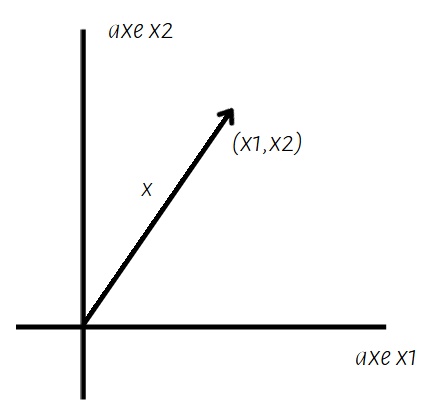
\includegraphics[scale=.45]{Chap1/vector1.png}\\
    \textit{Les éléments de $\R^2$ peuvent être vus comme des point ou des vecteurs.}
\end{center}
\noindent
Les axes et coordonnées explicites remplissent inutilement l'image ci-dessus, et on comprend souvent mieux en les supprimant et en pensant juste au vecteur, comme dans l'image ci-dessous.\\

\begin{center}
    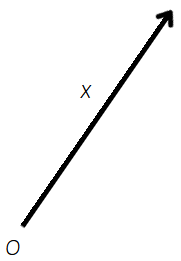
\includegraphics[scale=.45]{Chap1/vector2.png}\\
    \textit{Un vecteur}
\end{center}


Lorsque l'on utilise des images dans $\R^2$ ou le langage quelques peu vague des points et vecteurs, il faut se souvenir que ce ne sont que des aides à notre compréhension, et non pas des substituts pour les mathématiques effectives que nous allons développer. Même si nous ne pouvons dessiner de bonnes images dans des espaces à plus de dimensions, les éléments de ces dimensions sont définis aussi rigoureusement que ceux de $\R^2$. Par exemple, $(2,-3,17,\pi,\sqrt{2})$ est un élément de $\R^5$, et nous pouvons simplement nous référer à lui comme à un point ou un vecteur de $\R^5$ sans avoir à s'inquiéter de si la géométrie de $\R^5$ a le moindre sens physique.\\

\indent\marginpar{\flushleft{\textit{Les modèles mathématiques pour l'économie ont souvent des milliers de variables, par exemple $x_1,\ldots,x_{5000}$, ce qui veut dire que nous devons opérer dans $\R^{5000}$. Un tel espace ne peux pas être étudié géométriquement, mais l'approche algébrique fonctionne bien. C'est pour quoi notre sujet s'appelle l'\textbf{algèbre} linéaire.}}}
Souvenez-vous que nous définissons la somme de 2 éléments de $\K^n$ comme étant l'élément de $\K^n$ obtenue en additionnant les coordonnées correspondantes; comme vu en 0.0.1. Dans le cas particulier de $\R^2$, l'addition a une interprétation géométrique simple. Supposons que nous avons 2 vecteurs $x$ et $y$ dans $\R^2$ et que nous voulons les additionner, comme dans le côté gauche de l'image ci-dessous. Nous déplaçons le vecteur $y$ parallèle à lui-même pour que son origine coïncide avec l'extrémité de $x$. La somme $x+y$ est alors égale au vecteur dont l'origine correspond à celle de $x$ et l'extrémité à celle du nouveau vecteur $y$, comme sur le côté droit de l'image ci-dessous.\\

 

\begin{center}
    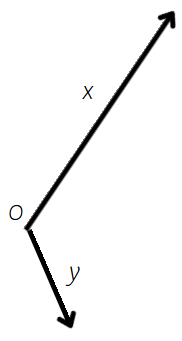
\includegraphics[scale=.45]{Chap1/2vectors.png}
    \hspace{1cm}
    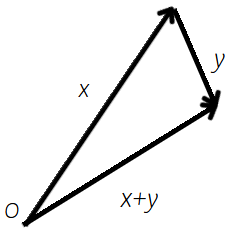
\includegraphics[scale=.45]{Chap1/2vectors2.png}\\
    \textit{La somme de 2 vecteurs}
\end{center}

Notre traitement du vecteur $y$ dans l'image ci-dessus illustre une philosophie standard lorsque nous pensons les vecteurs de $\R^2$ comme des flèches : nous pouvons les déplacer parallèles à elles-mêmes (sans changer leur longueur ou direction) et toujours avoir le même vecteur.\\
\indent
Maintenant que nous avons vu l'addition dans $\K^n$, nous nous tournons vers la multiplications. Nous pourrions définir la multiplication de manière similaire, en commançant avec 2 éléments de $\K^n$ et en en obtenant un nouveau en multipliant les coordonnées correspondantes. Cependant l'expérience nous montre que cette définition ne nous est pas utile. Un autre type de multiplication, appelé multiplication scalaire, sera centrale dans notre sujet. Spécifiquement, nous avons besoin de définir ce que veut dire multiplier un élément de $\K^n$ par un élément de $\K$. Nous choisissons la définition évidente : effectuer une multiplication sur chaque coordonné :
\begin{equation*}
    a(x_1,\ldots,x_n)=(ax_1,\ldots,ax_n)~;
\end{equation*}
ici $a\in\K$ et $(x_1,\ldots,x_n)\in\K^n$.\\
\indent
La multiplication scalaire a une belle interprétation géométrique dans $\R^2$. Si $a$ est un nombre positif et $x$ un vecteur de $\R^2$, alors $ax$ est le vecteur qui pointe dans la même direction que x et dont la longueur est $a$ fois celle de $x$. Autrement dit, pour obtenir $ax$, on rétrécit ou étire $x$ par un facteur $a$, en fonction de si $a<1$ ou $a>1$. La prochaine image illustre ceci.

\begin{center}
    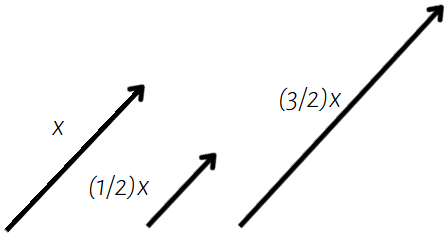
\includegraphics[scale=.45]{Chap1/PosMult.png}\\
    \textit{Multiplication par un scalaire positif}
\end{center}

\noindent
Si $a$ est un nombre négatif et $x$ un vecteur de $\R^2$, alors $ax$ est le vecteur qui pointe dans la direction opposée à $x$ et dont la longueur est $|a|$ fois la longueur de $x$, comme montré ci-dessous.

\begin{center}
    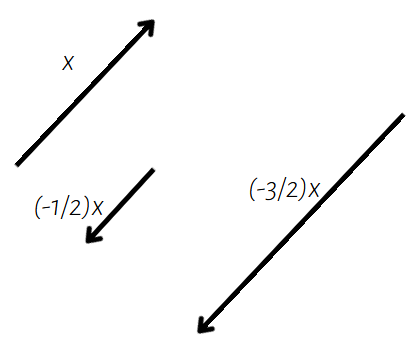
\includegraphics[scale=.45]{Chap1/NegMult.png}\\
    \textit{Multiplication par un scalaire négatif}
\end{center}

La motivation pour avoir défini un espace vectoriel vient des propriétés importantes de l'addition et de la multiplication scalaire de $\K^n$. En particulier, l'addition dans $\K^n$ est commutative et associative et possède un élément neutre, à savoir 0. Tout élément possède un opposé. La multiplication scalaire dans $\K^n$ est associative, et la multiplication scalaire par 1 fonctionne comme l’élément neutre. Enfin, l'addition et la multiplication dans $\K^n$ sont connectées par la distributivité.\\
\indent
Nous allons définir un espace vectoriel comme étant un ensemble $E$ ainsi qu'une addition et une multiplication scalaire dans $E$ qui satisfassent les propriétés énoncées dans le paragraphe précédent. Par une \textit{addition} sur $E$, nous voulons parler d'une fonction qui, à chaque paire d'éléments $u,v\in E$, assigne un élément $u+v$ dans $E$. Par une \textit{multiplication scalaire} dans $E$, nous voulons parler d'une fonction qui, à chaque $a\in\K$ et chaque $v\in E$, assigne un élément $av$ dans $E$.\\
\indent
Nous sommes désormais prêts pour donner une définition formelle d'un espace vectoriel. Un \textit{espace vectoriel} est un ensemble $E$ ainsi qu'une addition sur $E$ et qu'une multiplication scalaire sur $E$, tels que les propriétés suivantes s'appliquent :\\

\noindent
\textbf{Commutativité}\\
\indent{$u+v=v+u$ pour tous $u,v\in E$} ;\\

\noindent
\textbf{Associativité}\\
\indent{$(u+v)+w=u+(v+w)$ et $(ab)v=a(bv)$ pour tous $u,v,w\in E$ et tous\\
\indent $a,b\in\K$} ;\\

\noindent
\textbf{Élément neutre additif}\\
\indent{il existe un élément $0\in E$ tel que $v+0=v$ pour tout $v\in E$} ;\\

\noindent
\textbf{Opposé}\\
\indent{pour tout $v\in E$, il existe $w\in E$ tel que $v+w=0$} ;\\

\noindent
\textbf{Élément neutre multiplicatif}\\
\indent{$1v=v$ pour tout $v\in E$} ;\\

\noindent
\textbf{Distributivité}\\
\indent{$a(u+v)=au+av$ et $(a+b)v=av+bv$ pour tous $a,b\in\K$ et tous $u,v\in E$}.\\

\indent
La multiplication scalaire dans un espace vectoriel dépend de $\K$. De ce fait, si nous avons besoin d’être précis, nous dirons que $E$ est un espace vectoriel sur $\K$ au lieu de simplement dire que $E$ est un espace vectoriel. Par exemple, $\R^n$ est un espace vectoriel sur $\R$ et $\C^n$ est un espace vectoriel sur $\C$. Fréquemment, un espace vectoriel sur $\R$ est appelé un \textit{espace vectoriel réel} et un espace vectoriel sur $\C$ est appelé un \textit{espace vectoriel complexe}. Normalement, le choix de $\K$ est soit évident grâce au contexte, soit non pertinent, c'est pourquoi nous supposons souvent que $\K$ se cache en arrière-plan sans le mentionner spécifiquement.\\
\indent
Les éléments d'un espace vectoriel sont appelés \textit{vecteurs} ou \textit{points}. Ce langage géométrique aide parfois notre intuition.\\
\indent
Sans surprise, $\K^n$ est un espace vectoriel sur $\K$, comme vous devriez le vérifier. Naturellement, cet exemple a motivé notre définition d'espace vectoriel.\\
\indent\marginpar{\flushright{\textit{L'espace vectoriel le plus simple contient seulement 1 point. Autrement dit, \{0\} est un espace vectoriel, quoique très peu intéressant.}}}
Pour un autre exemple, considérez $\K^{\infty}$, qui est défini comme l'ensemble de toutes les séquences déléments de $\K$ :
\begin{equation*}
    \K^{\infty} = \{(x_1,x_2,\ldots):x_j\in\K \textrm{~pour~} j=1,2,\ldots\}.
\end{equation*}
L'addition et la multiplication scalaire sont définies sur $\K^{\infty}$ comme attendu :


%\begin{eqnarray*}
%        (x_1,x_2,\ldots)+(y_1,y_2,\ldots)=(x_&+y_1,x-2+y_2,\ldots)\\
%        a(x_1,x_2,\ldots)=(ax_1,ax_2,\ldots)
%\end{eqnarray*}

% Correction  Ne pas utiliser eqnarray voir https://www.tug.org/pracjourn/2006-4/madsen/madsen.pdf
\begin{equation*}
    (x_1,x_2,\ldots)+(y_1,y_2,\ldots)=(x_1+y_1,x-2+y_2,\ldots),
\end{equation*}
\begin{equation*}
    a(x_1,x_2,\ldots)=(ax_1,ax_2,\ldots).
\end{equation*}

Avec\marginpar{\flushright{\textit{Même si $\K^n$ est un exemple crucial d’espace vectoriel, tous les espaces vectoriels ne consistent pas de tuples. Par exemple, les éléments de $\mathcal{P}(\K)$ sont des fonctions sur $\K$ et non des tuples. En général. un espace vectoriel est une entité abstraite dont les éléments peuvent être des tuples, des fonctions, ou des objets étranges.}}} ces définitions, $\K^{\infty}$ devient un espace vectoriel sur $\K$, comme vous devriez le vérifier. L’élément neutre pour l'addition dans cet espace vectoriel est la séquence constituée uniquement de 0.\\
\indent
Notre prochain exemple est un espace vectoriel incluant des polynômes. Une fonction $p:\K\mapsto\K$ est appelée un \textit{polynôme} à coefficients dans $\K$ si il existe $a_0,\ldots,a_m\in\K$ tel que
\begin{equation*}
    p(z)=a_0+a_1z+a_2z^2+\ldots+a_mz^m
\end{equation*}
pour tout $z\in\K$. On définit $\mathcal{P}(\K)$ comme l’ensemble de tous les polynômes  à coefficients dans $\K$. L’addition dans $\mathcal{P}(\K)$ est définie comme vous vous y attendriez : si $p,q\in\mathcal{P}(\K)$, alors $p+q$ est le polynôme défini par
\begin{equation*}
    (p+q)(z)=p(z)+q(z)
\end{equation*}
pour $z\in\K$. Par exemple, si $p$ est le polynôme défini par $p(z)=2z+z^3$ et $q$ le polynôme défini par $q(z)=7+4z$, alors $p+q$ est le polynôme défini par $(p+q)(z)=7+6z+z^3$. La multiplication scalaire sur $\mathcal{P}(\K)$ a également une définition évidente : si $a\in\K$ et $p\in\mathcal{P}(\K)$, alors $ap$ est le polynôme défini par
\begin{equation*}
    (ap)(z)=ap(z)
\end{equation*}
pour $z\in\K$. Avec ces définitions de l’addition et de la multiplications scalaire, $\mathcal{P}(\K)$ est un espace vectoriel, comme vous devriez le vérifier. L’élément neutre additif dans cet espace vectoriel est le polynôme dont tous les coefficients sont égaux à 0.\\
\indent
Bientôt nous verrons d’autres exemples d’espace vectoriel, mais nous devons d’abord développer certaines des propriétés élémentaires des espaces vectoriels.\\


\section*{Propriétés des espaces vectoriels}

La définition d'un espace vectoriel requiert que ce dernier ait un élément neutre additif. La proposition ci-dessous énonce que cet élément est unique.\\

\begin{prop}
    Un espace vectoriel a un élément neutre additif unique.
    \begin{proof}
        Supposons que 0 et 0' sont tous deux des élément neutres d'un espace vectoriel $E$. Alors 
        \begin{equation*}
            0'=0'+0=0,
        \end{equation*}
        où la première équation vient du fait que 0 est un élément neutre, et la deuxième parce que 0' est aussi un élément neutre. Ainsi, $0=0'$, ce qui montre que $E$ ne possède qu'un seul élément neutre additif.\marginpar{\flushleft{\textit{Le symbole $\blacksquare$ signifie <<fin de la preuve>>.}}}
    \end{proof}
\end{prop}

Chaque élément $v$ d'un espace vectoriel a un opposé, un élément $w$ dans l'espace vectoriel teel que $v+w=0$. La proposition ci-dessous énonce que chaque élément dans un espace vectoriel a un unique opposé.\\

\begin{prop}
    Chaque élément dans un espace vectoriel a un unique opposé.
    \begin{proof}
        Supposons que $E$ est un espace vectoriel avec $v\in E$. Supposons que $u$ et $w$ sont des opposés de $v$. Alors
        \begin{equation*}
            u=u+0=u+(v+w)=(u+v)+w=0+w=w.
        \end{equation*}
        Ainsi, $u=w$ comme désiré.
    \end{proof}
\end{prop}

Maintenant que nous savons que l'opposé est unique, pour $v$ un élément d'un espace vectoriel, on peut noter $-v$ l'opposé de $v$. On définit $w-v$ comme signifiant $w+(-v)$.\\
\indent
Presque tous les résultats de ce livre vont inclure des espaces vectoriels. Pour éviter d'être distrait par le fait d'avoir à redire sans arrêt une phrase comme <<Supposons que $E$ est un espace vectoriel>>, nous allons maintenant faire la déclaration nécessaire une fois pour toutes :

\begin{center}
    \begin{tabular}{|c|}
        \hline
        Mettons-nous d'accord que pour le reste du livre,   \\
        $E$ désignera un espace vectoriel sur $\K$.   \\
        \hline
    \end{tabular}
\end{center}

Grâce à l'associativité, nous pouvons oublier les parenthèses lorsque nous manipulons des additions à plus de 2 éléments dans un espace vectoriel. Par exemple, nous pouvons écrire $u+v+w$ sans parenthèses puisque les 2 interprétations possibles de cette expressions, à savoir $(u+v)+w$ et $u+(v+w)$, sont égales. Nous utliserons cette conventions familière de ne pas utiliser de parenthèses dans la prochaine preuve. Dans la prochaine proposition, 0 désigne un scalaire (le nombre $0\in\K$) du côté gauche de l'équation et un vecteur (l'élément neutre additif de $E$) du côté droit de l'équation.\\

\marginpar{\flushright{\textit{Notez que 1.4 et 1.5 parlent de la multiplication scalaire et de l'élément neutre additif de $E$. La seule partie de la définition d'un espace vectoriel qui relie la multiplication scalaire et l'addition de vecteurs est la distributivité. De ce fait, la distributivité doit être utilisée dans les preuves.}}}
\begin{prop}
    $0v=0$ pour tout $v\in E$.
    \begin{proof}
        Pour $v\in E$, nous avons
        \begin{equation*}
            0v=0v+0v-0v=(0+0)v-0v=0v-0v=0,
        \end{equation*}
        comme voulu.
    \end{proof}
\end{prop}

Dans la prochaine proposition, 0 désignera l'élément neutre additif de $E$. Même si leur preuves sont similaires, 1.4 et 1.5 ne sont pas identiques. Plus précisément, 1.4 dit que le produit du scalaire 0 avec n'importe quel vecteur est égal au vecteur 0, tandis que 1.5 dit que le produit de n'importe quel scalaire avec le vecteur 0 donne le vecteur 0.\\

\begin{prop}
    $a0=0$ pour tout $a\in\K$.
    \begin{proof}
        Pour $a\in\K$, on a
        \begin{equation*}
            a0=a0+a0-a0=a(0+0)-a0=a0-a0=0,
        \end{equation*}
        comme voulu.
    \end{proof}
\end{prop}

Maintenant nous allons montrer que si un élément de $E$ est multiplié par le scalaire $-1$, alors le résultat est l'opposé de l'élément de $E$.

\begin{prop}
    $(-1)v=-v$ pour tout $v\in E$.
    \begin{proof}
        Pour $v\in E$, on a
        \begin{equation*}
            v+(-1)v=1v+(-1)v=(1+(-1))v=0v=0,
        \end{equation*}
        Cette équation dit que $(-1)v$, quand il est additionné à $v$, donne 0. De ce fait, $(-1)v$ doit être l'opposé de $v$, comme voulu.
    \end{proof}
\end{prop}

\section*{Sous-espaces vectoriels}

Un {\marginpar{\flushleft{\textit{Certains mathématiciens utilisent le terme \textbf{sous-espace linéaire}, ce qui veut dire la même chose que sous-espace vectoriel}}}} sous-ensemble $F$ de $E$ est appelé \textit{sous-espace vectoriel} de $E$ si $F$ est également un espace vectoriel (en utilisant les mêmes addition et multiplication scalaire que dans $E$). Par exemple,
\begin{equation*}
    \{(x_1,x_2,0):x_1,x_2\in\K\}
\end{equation*}
est un sous-espace vectoriel de $\K^3$. Si $F$ est un sous-ensemble de $E$ non vide, alors pour vérifier que $F$ est un sous-espace vectoriel de $E$, nous avons seulement besoin de vérifier que $F$ satisfait les propriétés suivantes :\\

\noindent
\textbf{Stabilité pour l'addition}\\
\indent{$u,v\in F$ implique que $u+v\in F$}\\

\noindent
\textbf{Stabilité pour la multiplication scalaire}\\
\indent{$a\in\K$ et $u\in F$ implique que $au\in F$}\\

\noindent
La première condition {\marginpar{\flushleft{\textit{Il est évident que \{0\} est le plus petit sous-espace vectoriel de $E$ et que $E$ lui-même est le plus grand. L'ensemble nul n'est pas un sous-espace vectoriel de $E$ parce qu'un sous-espace vectoriel doit être un espace vectoriel et qu'un espace vectoriel doit contenir au moins un élément, à savoir un élément neutre additif.}}}}, qui peut être décrite en disant que $F$ est \textit{fermé sous l'addition}, assure que l'addition a un sens dans $F$. La seconde, qui peut être décrite en disant que $F$ est \textit{fermé sous la multiplication scalaire}, assure que la multiplication scalaire a un sens dans $F$. Pour montrer que $F$ est un espace vectoriel, les autres parties de la définition d'un espace vectoriel n'ont pas besoin d’être vérifiées, car elles sont automatiquement satisfaites. Par exemple, l'associativité et la commutativité de l'addition sont automatiquement valables dans $F$ car elles le sont dans le plus grand espace $F$. Pour donner un autre exemple, si la seconde condition ci-dessus est vraie et que $u\in F$, alors $-u$ (qui est égal à $(-1)u$ par 1.6), est également dans $F$, et de ce fait tout élément de U a un opposé dans $F$.\\
\indent
Les 2 conditions ci-dessus nous permettent généralement de déterminer rapidement si un sous-ensemble de $E$ donné est ou non un sous-espace vectoriel de $E$. Par exemple, si $b\in\K$, alors
\begin{equation*}
    \{(x_1,x_2,x_3,x_4)\in\K^4:x_3=x_4+b\}
\end{equation*}
est un sous-espace vectoriel de $\K^4$ si, et seulement si $b=0$, comme vous devriez le démontrer. Pour un autre exemple, vous devriez démontrer que
\begin{equation*}
    \{p\in \mathcal{P}(\K):p(3)=0\}
\end{equation*}
est un sous-espace vectoriel de $\mathcal{P}(\K)$.\\
\indent
Les sous-espaces vectoriels de $\R^2$ sont précisément \{0\}, $\R^2$, et toutes les lignes de $\R^2$ passant par l'origine. Les sous-espaces vectoriels de $\R^3$ sont précisément \{0\}, $\R^3$, toutes les lignes de $\R^3$ passant par l'origine, et tous les plans de $\R^3$ passant par l'origine. Prouver que tous ces objets sont en effet des sous-espaces vectoriels est simple---la partie compliquée est de montrer que ce sont les seuls sous-espaces vectoriels de $\R^2$ ou de $\R^3$. Cette tâche sera plus simple après avoir introduit quelques outils supplémentaires dans le chapitre suivant.

\section*{Sommes et sommes directes}
Dans des chapitres futurs, nous trouverons que les notions de somme et somme directe d'espace vectoriel sont utiles. Nous allons donc ici définir ces concepts.\\
\indent
Supposons que $F_1,\ldots,F_m$ sont des sous-espaces vectoriels de $E$. La \textit{somme} de $F_1,\ldots,F_m$, notée $F_1+\ldots+F_m$, est définie comme l'ensemble de toutes les sommes possibles d'éléments de $F_1,\ldots,F_m$. Plus précisément,
\begin{equation*}
    F_1+\ldots+F_m=\{u_1+\ldots+u_m:u_1\in F_1,\ldots,u_m\in F_m\}
\end{equation*}

Vous devriez vérifier que si $F_1,\ldots,F_m$ sont des sous-espaces vectoriels de $E$, alors la somme $F_1+\ldots+F_m$ est un sous-espace vectoriel de $E$. \marginpar{\flushleft{\textit{Lorsque l'on manipule des espaces vectoriels, nous sommes généralement seulement intéressés par les sous-espaces vectoriels, et non pas par des sous-ensembles arbitraires. L'union d'espace vectoriels est rarement un espace vectoriel (voir l'exercice 9 de ce chapitre), c'est pourquoi nous travaillons surtout avec des sommes plutôt que des unions.}}}\\

Regardons quelques exemples de somme de sous-espaces vectoriels. Supposons que $F$ est l'ensemble de tous les éléments de $\K^3$ dont la deuxième et troisième coordonnée est égale à 0, et que $E$ est l'ensemble de tous les éléments de $\K^3$ dont la première et troisième coordonnée est égale à 0 :
\begin{equation*}
    F=\{(x,0,0)\K^3:x\in\K\} \textrm{~et~} G=\{(0,y,0)\K^3:y\in\K\}
\end{equation*}
Alors
\begin{prop}
    \begin{equation*}
        F+G=\{(x,y,0):x,y\in\K\}
    \end{equation*}
\end{prop}
comme vous devriez le vérifier.\\
\indent
Pour un autre exemple, supposez que $F$ est défini comme ci-dessus, et que $G$ est l'ensemble de tous les élément de $\K^3$ dont la première et la deuxième coordonnée sont égales, et la troisième vaut 0 :
\begin{equation*}
    G=\{(y,y,0)\K^3:y\in\K\}
\end{equation*}
Alors $F+G$ est aussi donné par 1.7, comme vous devriez le vérifier.\\

\indent
\marginpar{\flushright{\textit{Les sommes d'espaces vectoriels en théorie des espaces vectoriels sont analogues aux unions d'ensembles en théorie des ensemble. Si on a 2 sous-espaces vectoriels d'un espace vectoriel, le plus petit sous-espace vectoriel contenant les 2 premiers est leur somme. Analoguement, si on a 2 sous-ensemble d'un ensemble, le plus petit sous-ensemble les contenant est leur somme.}}}Supposons que $F_1,\ldots,F_m$ sont des sous-espaces vectoriels de $E$. évidemment, $F_1,\ldots,F_m$ sont tous contenus dans $F_1+\ldots+F_m$ (pour voir cela, considérez la somme $u_1+\ldots+u_m$ où tous les $u$ sauf 1 valent 0). à l'inverse, tout sous-espace vectoriel de $E$ contenant $F_1,\ldots,F_m$ doit contenir $F_1+\ldots+F_m$ (puisqu'un sous-espace vectoriel doit contenir toutes les sommes finies de ses éléments). De ce fait, $F_1+\ldots+F_m$ est le plus petit sous-espace vectoriel de $V$ contenant $F_1,\ldots,F_m$.\\

Supposons que $F_1,\ldots,F_m$ sont des sous-espaces vectoriels de $E$ tels que $E=F_1+\ldots+F_m$. De ce fait, tout élément de $E$ peut être écrit sous la forme
\begin{equation*}
    u_1+\ldots+u_m
\end{equation*}
où chaque $u_j\in F_j$. Nous serons en particulier intéressés par les cas où chaque vecteur de $F$ peut être représenté de manière unique sous la forme ci-dessus. Cette situation est tellement importante que nous lui donnons un nom particulier : une somme directe. En particulier, nous disons que $F$ est la \textit{somme directe} des sous-espaces vectoriels $F_1,\ldots,F_m$, écrit $E=F_1\oplus\ldots\oplus F_m$, si chaque élément de $V$ peut être écrit de manière unique comme une somme $u_1+\ldots+u_m$ où chaque $u_j\in F_j$.\\

Regardons quelques exemples de somme directe. Supposons que $F$ est le sous-espace vectoriel de $\K^3$ constitué de ses vecteurs dont la dernière coordonnée vaut 0, et $G$ le sous-espace vectoriel de $\K^3$ constitué de ses vecteurs dont la première et deuxième coordonnée vaut 0 :
\begin{equation*}
    U=\{(x,y,0)\in\K^3:x,y\in\K\} \textrm{~et~} W=\{(0,0,z)\in\K^3:z\in\K\}
\end{equation*}
Alors $\K^3=F\oplus G$, comme vous devriez le vérifier.\\

Comme autre exemple, supposons que $F_j$ est le sous-espace vectoriel de $\K^n$ constitué de ses vecteurs dont toutes les coordonnées valent 0, exceptées possiblement en $j\ieme$ position (par exemple, $F_2=\{(0,x,0,\ldots,0)\in\K^n:x\in\K\}$). Alors on a
\begin{equation*}
    \K^n=F_1\oplus\ldots\oplus F_n
\end{equation*}
comme vous devriez le vérifier.\marginpar{\flushleft{\textit{Le symbole $\oplus$, constitué d'un signe plus à l'intérieur d'un cercle, est utilisé pour rappeler que nous travaillons avec un type particulier de somme de sous-espaces vectoriels---chaque élément dans une somme directe peut être représenté de manière unique comme une somme d'éléments des sous-espaces vectoriels sommés.}}}\\

Pour notre dernier exemple, considérons l'espace vectoriel $\mathcal{P}(\K)$ de tous les polynômes à coefficient dans $\K$. $F_p$ désigne le sous-espace vectoriel de $\mathcal{P}(\K)$ constitué de tous les polynômes $p$ de la forme
\begin{equation*}
    p(z)=a_0+a_2z^2+\ldots+a_{2m}z^{2m}
\end{equation*}
et $F_i$ désigne le sous-espace vectoriel de $\mathcal{P}(\K)$ constitué de tous les polynômes $p$ de la forme
\begin{equation*}
    p(z)=a_1z+a_3z^3+\ldots+a_{2m+1}z^{2m+1}
\end{equation*}
ici $m$ est un entier positif, et $a_0,\ldots,a_{2m+1}\in\K$ (les notations $F_p$ et $F_i$ devraient vous rappeler le puissances paires et impaires de $z$). Vous devriez vérifier que
\begin{equation*}
    \mathcal{P}(\K)=F_p\oplus F_i
\end{equation*}

Parfois un contre-exemple nous aide à comprendre autant qu'un exemple. Considérez les 3 sous-espaces vectoriels suivants de $\K^3$ :
\begin{eqnarray*}
    F_1=\{(x,y,0)\in\K^3:x,y\in\K\}\\
    F_2=\{(0,0,z)\in\K^3:z\in\K\}\\
    F_3=\{(0,y,y)\in\K^3:y\in\K\}\\
\end{eqnarray*}
Clairement $\K^3=F_1+F_2+F_3$ car un vecteur arbitraire $(x,y,z)\in\K^3$ peut être écrit sous la forme
\begin{equation*}
    (x,y,z)=(x,y,0)+(0,0,z)+(0,0,0)
\end{equation*}
où le premier vecteur du côté droit appartient à $F_1$, le deuxième à $F_2$ et le troisième à $F_3$. Cependant $\K^3$ n'est pas égal à la somme directe de $F_1,F_2,F_3$ car le vecteur $(0,0,0)$ peut être écrit de 2 façon différentes comme une somme $u_1+u_2+u_3$, avec chaque $u_j\in F_j$. Spécifiquement, on a
\begin{equation*}
    (0,0,0)=(0,1,0)+(0,0,1)+(0,-1,-1)
\end{equation*}
et, évidemment,
\begin{equation*}
    (0,0,0)=(0,0,0)+(0,0,0)+(0,0,0)
\end{equation*}
où le premier vecteur du côté droit de chaque équation appartient à $F_1$, le deuxième à $F_2$ et le troisième à $F_3$.\\
\indent
Dans l'exemple ci-dessus, on a montré que nous n'avions pas de somme directe en montrant que 0 n'avait pas de représentation unique comme une somme de vecteurs appropriés. La définition d'une somme directe requiert que chaque vecteur dans l'espace ait une unique représentation comme une somme appropriée. Supposons que nous ayons une collection de sous-espaces vectoriels dont la somme vaut l'espace vectoriel entier. La prochaine proposition montre que lorsque l'on cherche si cette collection de sous-espaces vectoriels est une somme directe, nous avons seulement besoin de vérifier si 0 peut être exprimé de manière unique.

\begin{prop}
    Supposons que $F_1,\ldots,F_n$ sont des sous-espaces vectoriels de $E$. Alors $E=F_1\oplus\ldots\oplus F_n$ si, et seulement si, les conditions suivantes sont respectées :
    \begin{description}
        \item[(a)] $ E=F_1+\ldots+F_n $
        \item[(b)] le seul moyen d'écrire 0 comme une somme $u_1+\ldots+u_n$ où chaque $u_j\in F_j$ est de prendre chaque $u_j$ égal à 0
    \end{description}
\end{prop}

\textsc{Preuve :} Supposons d'abord que $E=F_1\oplus\ldots\oplus F_n$. évidemment (a) est vérifié (cela vient de comme la somme et la somme directe sont définies). Pour prouver (b), supposons que $u_1\in F_1,\ldots,u_n\in F_n$ et
\begin{equation*}
    0=u_1+\ldots+u_n
\end{equation*}
Alors chaque $u_j$ doit valoir 0 (cela vient de l'unicité dans la définition de la somme directe, car $0=0+\ldots+0$ et $0\in F_1,\ldots,0\in F_n$), ce qui prouve (b).\\
\indent
Maintenant, supposons que (a) et (b) sont vrais. Soit $v\in E$. Par (a), nous pouvons écrire $v=u_1+\ldots+u_n$ avec $u_1\in F_1,\ldots,u_n\in F_n$. Pour montrer que cette représentation est unique, supposons que nous avons également $v=v_1+\ldots+v_n$ avec $v_1\in F_1,\ldots,v_n\in F_n$. En soustrayant les deux équations, on obtient
\begin{equation*}
    0=(u_1-v_1)+\ldots+(u_n-v_n)
\end{equation*}
\indent Clairement, $u_1-v_1\in F_1,\ldots,u_n-v_n\in F_n$, donc l'équation ci-dessus et (b) impliquent que chaque $u_j-v_j=0$. Ainsi, $u_1=v_1,\ldots,u_n=v_n$, comme voulu. \hfill$\blacksquare$

La prochaine proposition donne une condition simple pour tester quelles paires de sous-espaces vectoriels donne une somme directe. Notez que cette proposition traite seulement du cas avec 2 sous-espaces vectoriels. Lorsque vous vous demandez si la somme de plus de 2 sous-espaces vectoriels est directe, il n'est pas suffisant de tester si n'importe quelle paire de sous-espaces vectoriels s'intersectent seulement en 0. Pour voir cela, considérez le contre-exemple présenter juste avant 1.8. Dans ce contre-exemple nous avions $\K^3=F_1+F_2+F_3$, mais $\K^3$ n'étais pas égal à la somme directe de $F_1,F_2,F_3$. Cependant, dans ce contre-exemple, Nous avons $F_1 \cap F_2=F_2 \cap F_3=F_3 \cap F_1=\{0\}$ (comme vous devriez le vérifier). La prochaine proposition montre qu'avec seulement 2 sous-espaces vectoriels nous avons une condition nécessaire et suffisante pour qu'un somme soit directe.


\begin{prop}
    Supposons\marginpar{\flushleft{\textit{La somme de sous-espaces vectoriels est analogue à l'union de nous-ensembles. Similairement, la somme directe est analogue à l'union disjointe de sous-ensembles. Bien sûr, 2 sous-espaces vectoriels ne peuvent être disjoint, car ils doivent tous deux contenir 0. Donc la disjointness est remplacée, au moins pour le cas de 2 sous-espaces vectoriels, par la contrainte que l'intersection égale \{0\}.}}} que $F$ et $G$ soient des sous-espaces vectoriels de $E$. Alors $E=F\oplus G$ si, et seulement si, $E=F+G$ et $F \cap G=\{0\}$.
\end{prop}
\textsc{Preuve :} Supposons d'abord que $E=F\oplus G$. Alors $E=F+G$ (par la définition d'une somme directe). De plus, si $v\in F \cap G$, alors $0=v+(-v)$, où $v\in F$ et $-v\in F$. Par l'unicité de la représentation de 0 comme la somme d'un vecteur dans $F$ et d'un vecteur dans $G$, nous devons avoir $v=0$. De ce fait, $F\cap G=\{0\}$, ce qui finit la preuve dans un sens.\\
\indent
Pour prouver la proposition dans l'autre sens, supposons maintenant que $E=F+G$ et $F\cap G=\{0\}$. Pour prouver que $E=F\oplus G$, supposons que
\begin{equation*}
    0=u+w
\end{equation*}
où $u\in F$ et $w\in G$. Pour compléter la preuve, nous avons seulement besoin de montrer que $u=w=0$ (par 1.8). L'équation ci-dessus implique que $u=-w\in G$. Ainsi $u\in F\cap G$, et donc $u=0$. Ceci, accompagné de l'équation ci-dessus, implique que $w=0$, ce qui complète la preuve. \hfill$\blacksquare$.





% A ajouter vers la ligne 460 : \marginpar{\Klushleft{\textit{Le symbole $\oplus$, constitué d'un signe plus à l'intérieur d'un cercle, est utilisé pour rappeler que nous travaillons avec un type particulier de somme de sous-espaces vectoriels---chaque élément dans une somme directe peut être représenté de manière unique comme une somme d'éléments des sous-espaces vectoriels sommés.}}}%
\end{document}
\newpage
\documentclass[12pt]{book}
\usepackage{stylepackage}

\begin{document}
\section*{Exercices}

\begin{enumerate}
    \item Supposez que $a$ et $b$ sont des nombres réels, non tous nuls. Trouver les nombres réels $c$ et $d$ tels que
    \begin{equation*}
        1/(a+ib)=c+id
    \end{equation*}
    \item Montrez que
    \begin{equation*}
        z=\frac{-1+i\sqrt{3}}{2}
    \end{equation*}
    est une racine cubique de 1 (ce qui veut dire que son cube vaut 1).
    \item Prouvez que si $a\in\F,~v\in E$, et que $av=0$, alors $a=0$ ou $v=0$.
    \item Prouvez que $-(-v)=v$ pour tout $v\in E$
    \item Pour chacun des sous-ensembles de $\F^3$ suivants, déterminez s'il s'agit d'un sous-espace vectoriel de $\F^3$ ou non :
    \begin{description}
        \item[(a)] $ \{(x_1,x_2,x_3)\in\F^3:x_1+2x_2+3x_3=0\} $
        \item[(b)] $ \{(x_1,x_2,x_3)\in\F^3:x_1+2x_2+3x_3=4\} $
        \item[(c)] $ \{(x_1,x_2,x_3)\in\F^3:x_1x_2x_3=0\} $
        \item[(d)] $ \{(x_1,x_2,x_3)\in\F^3:x_1=5x_3\} $
    \end{description}
    \item Prouvez que l'intersection de n'importe quel ensemble de sous-espace vectoriel de $E$ est un sous-espace vectoriel de $E$.
    \item Donnez un exemple d'un sous-ensemble $F$ de $\R^2$ non vide tel que $F$ soit stable pour l’addition et ait un opposé (c'est-à-dire que $-u\in F$ si $u\in F$), mais que $F$ n'est pas un sous-espace vectoriel de $\R^2$.
    \item Donnez un exemple d'un sous-ensemble $F$ de $\R^2$ non vide tel que $F$ soit stable pour la multiplication scalaire, mais que $F$ n'est pas un sous-espace vectoriel de $\R^2$.
    \item Prouvez que l'union de 2 sous-espaces vectoriels de $E$ est un sous-espace vectoriel de $E$ si seulement l'un des sous-espaces vectoriels est inclus dans l'autre.
    \item Supposez que $F$ est un sous-espace vectoriel de $E$. Qu'est-ce que $F+F$ ?
    \item Est-ce que l'opération d'addition sur les sous-espaces vectoriels de $F$ possède un élément neutre ? Quels sous-espaces vectoriels ont un opposé ?
    \item Prouvez ou donnez un contre-exemple : si $F_1, F_2,G$ sont des sous-espaces vectoriels de $E$ tels que
    \begin{equation*}
        F_1+G=F_2+G
    \end{equation*}
    alors $F_1=F_2$.
    \item Est-ce que l'addition sur des sous-espaces vectoriels de $E$ est commutative ? Associative ? (Autrement dit, si $F_1,F_2,F_3$ sont des sous-espaces vectoriels de $E$, est-ce que $F_1+F_2=F_2+F_1$ ? Est-ce que $(F_1+F_2)+F_3=F_1+(F_2+F_3)$ ?)
    \item Supposez que $F$ est le sous-espace vectoriel de $\mathcal{P}(\F)$ constitué de tous les polynômes $p$ de la forme
    \begin{equation*}
        p(z)=az^2+bz^5
    \end{equation*}
    où $a,b\in\F$. Trouvez un sous-espace vectoriel $G$ de $\mathcal{P}(\F)$ tel que $\mathcal{P}(\F)=F\oplus G$.
    \item Prouvez ou donnez un contre-exemple : si $F_1,F_2,G$ sont des sous-espaces vectoriels de $E$ tels que
    \begin{equation*}
        E=F_1\oplus G \mathrm{~et~} E=F_2\oplus G
    \end{equation*}
    alors $F_1=F_2$.
\end{enumerate}

















\end{document}
\newpage
\documentclass[12pt]{book}
\usepackage{stylepackage}

\begin{document}
%\thispagestyle{plain}%
\chapter{\textmd{\textsc{\Large{Chapitre 2}}} \\ \textsl{Espaces Vectoriels de// Dimension Finie}}

\vfill

\indent{Dans le dernier chapitre, nous avons appris les espaces vectoriels. L'alg\`ebre linéaire ne se concentre pas sur des espaces vectoriels arbitraires, mais sur des espaces vectoriels de dimension finie, que nous introduisons dans ce chapitre. Nous traiterons les concepts cl\'es associés à ces espaces: vect, ind\'ependance lin\'eaire, base et dimension.}

\indent{Passons en revue nos hypothèses de base :}
\begin{center}
\fbox{
\begin{minipage}{0.7 \textwidth }
\hspace{1 cm}Rappelons que $\K$ d\'esigne \bm{$R$} ou \bm{$C$}.\\
Rappelons aussi que $V$ est un espace vectoriel sur $\K$.\\ 
\end{minipage}
}
\end{center}
\vfill
\begin{center}

\includegraphics[scale=0.10]{Asterisk.png}
\hspace{1cm} 

\includegraphics[scale=0.10]{Asterisk.png}
\hfill 
\end{center}

\pagebreak
\newpage
%\begin{enumerate}%
\section*{\textsl{Famille et Ind\'ependance lin\'eaire}}
La combinaison lin\'eaire d'une famille $ (V_1,\ldots,V_m)$ de vecteur dans $V$ de la forme 


\noindent
\textbf{2.1}\hspace{3cm} $a_1V_1+\ldots+a_mV_m$ , 

 
\marginpar{\flushright{\textit{Certains math\'ematiciens utilisent le terme de \textbf{g\'en\'eratrice}, ce qui signifie la m\^eme chose que le vect.}}}
où $a_1,\ldots,a_m $ $\in \K$.L'ensemble de toutes les combinaisons lin\'eaires de $(V_1,\ldots,V_m)$ est appel\'e \textbf{vect} de $(V_1,\ldots,V_m)$. En d'autres termes,
\begin{equation*}
vect(V_1,\ldots,V_m)=\{a_1V_1+\ldots+a_mV_m : a_1,\ldots,a_m \in \K\}.
\end{equation*}
\hspace{0.5cm}\`A titre d’exemple de ces concepts, supposons que $V = \K^3$ .Le vecteur $(7,2,9)$ est une combinaison lin\'eaire de $((2,1,3),(1,0,1))$ parce que 
\begin{equation*}
(7,2,9)=2(2,1,3) + 3(1,0,1).
\end{equation*}
Ainsi $(7,2,9) \in vect ((2,1,3), (1,0,1)).$\\
\indent
Vous devez vérifier que le vect de toute famille de vecteurs dans $V$ est un sous-espace de $V$ . Pour être cohérent, nous déclarons que le vect de l'ensemble vide $()$ \'egal \{$0$\} (rappelez-vous que l’ensemble vide n’est pas un sous-espace de $V$).\\
\indent
Si $(V_1,\ldots,V_m)$ est une famille de vecteurs dans $V$, alors chaque $V_j$ est une combinaison lin\'eaire de $(V_1,\ldots,V_m)$ (pour montrer cela, d\'efinissez $a_j$=1 et laissez les autres $a$ dans 2.1 \'egal \`a 0).Ainsi vect$(V_1,\ldots,V_m)$ contient chaque $v_j$. Inversement, parce que les sous-espaces sont ferm\'es sous multiplication scalaire et addition, tout sous-espace de $V$ contenant chaque $v_j$ doit contenir vect$(V_1,\ldots,V_m)$. Ainsi, le vect d’une famille de vecteurs dans $V$ est le plus petit sous-espace de V contenant tous les vecteurs de la famille.\\
\indent
Si vect$(V_1,\ldots,V_m)$ \'egal $V$, nous disons que $(V_1,\ldots,V_m)$ \textbf{engendre} $V$.Un espace vectoriel est appel\'e \textbf{dimension finie} si quelques familles de vecteurs qu'il contient couvre l'espace. Par exemple, $\K^n$ est une dimension finie parce que 
\marginpar{\flushright{\textit{Rappelons que, par d\'efinition, chaque famille a une longueur finie.}}}
\begin{equation*}
((1,0,\ldots,0),(0,1,0,\ldots,0),(0,\ldots,0,1))
\end{equation*}
vects {$F^n$}, comme vous devriez le v\'erifier.\\
\indent 
Avant de donner l’exemple suivant d’un espace vectoriel de dimension finie, nous devons d\'efinir le degr\'e d’un polyn\^ome. Un polyn\^ome $p \in P(\K)$ est dit avoir un degr\'e $m$ s’il existe des scalaires $a_0,a_1,\ldots,a_m $ $\in  \K$ avec $a_m \ne$ $0$ tel que
\begin{equation*}
 p(z) = a_0 + a_1z +\ldots+ a_mz^m   
\end{equation*}


\pagebreak
\newpage
Pour tous les $z \in \K$. Le polynôme qui est identiquement $0$ est dit avoir un degr\'e $-\infty$.\\
\indent
Pour m un entier non n\'egatif, soit $P_m(\K)$ l’ensemble de tous les polyn\^omes ayant des coefficients en $\K$ et un degr\'e au plus $m$. Vous devez v\'erifier que $P_m(\K)$ est un sous-espace de $P(\K)$ ; par cons\'equent, $P_m(\K)$ est un espace vectoriel. Cet espace vectoriel est de dimension finie car il est couvert par la famille $(1,z,\ldots,z^m)$; ici, nous abusons l\'eg\`erement de la notation en laissant $z^k$ désigner une fonction (de même qu’une variable factice).\\
\marginpar{\flushleft{\textit{Les espaces vectoriels de dimension infinie, que nous ne mentionnerons plus beaucoup, sont le centre d’attention dans la branche des math\'ematiques appel\'ee \textbf{analyse fonctionnelle}. L’analyse fonctionnelle utilise des outils d’analyse et d’alg\`ebre.}}}
\indent
Un espace vectoriel qui n’est pas de dimension finie est appel\'e \textbf{dimension infinie}. Par exemple, $P(\K)$. Pour le prouver, consid\'erez n’importe quelle famille d’\'el\'ements de $P(\K)$. Soit $m$ le degr\'e le plus \'elev\'e de l’un des polyn\^omes de la famille consid\'er\'ee (rappelons que par d\'efinition une famille a une longueur finie). Ensuite, chaque polyn\^ome dans le vect de cette liste doit avoir un degr\'e au plus $m$. Ainsi, notre famille ne peut pas engendrer $P(\K)$.  \'Etant donn\'e qu’aucune famille n'engendre $P(\K)$, cet espace vectoriel est de dimension infinie.\\
\indent
L’espace vectoriel $\K^\infty$, compos\'e de toutes les s\'equences d’\'el\'ements de $\K$, est \'egalement de dimension infinie, bien que cela soit un peu plus difficile \'a prouver. Vous devriez \^etre en mesure de donner une preuve en utilisant certains des outils que nous allons bient\^ot d\'evelopper.\\
\indent
Supposons $v_1,\ldots,v_m$ en $V$ et $V$ en vect$(v_1,\ldots,v_m)$. Par la d\'efinition de vect, il existe $a_1,\ldots,a_m \in \K$ tel que
\begin{equation*}
V = a_1V_1+\ldots+a_mV_m.
\end{equation*}
Examiner la question de savoir si le choix de a dans l’\'equation ci-dessus est unique. Supposons que $\hat{a}_1,\ldots,\hat{a}_m$ soit un autre ensemble de scalaires tels que
\begin{equation*}
    V = \hat{a}_1v_1,\ldots,\hat{a}_mv_m.
\end{equation*}
En soustrayant les deux derni\`eres \'equations, nous avons
\begin{equation*}
    0 =(a_1 - \hat{a}_1)v_1+\ldots+(a_m - \hat{a}_m)v_m.
\end{equation*}
Ainsi, nous avons \'ecrit $0$ comme combinaison lin\'eaire de $(v_1,\ldots,v_m)$. Si la seule façon de le faire est la mani\`ere \'evidente (en utilisant $0$ pour tous les scalaires), alors chaque $a_j - \hat{a}j$ est \'egal \`a $0$, ce qui signifie que chaque $a_j$ est \'egal \`a $\hat{a}j$ (et donc le choix de a \'etait en effet unique). Cette situation est si importante que nous lui donnons un nom sp\'ecial -- l’ind\'ependance lin\'eaire -- que nous d\'efinissons maintenant.\\
\pagebreak
\indent
Une famille $(v_1,\ldots,v_m) $de vecteurs est dit \textbf{libre} si le seul choix de $a_1,\ldots,a_m$ dans $\K$ qui rend $a_1V_1+\ldots+a_mV_m$ \'egal $0$ est $a_1 = \ldots = a_m = 0$. Par exemple,
\begin{equation*}
((1,0,0,0),(0,1,0,0),(0,0,1,0))
\end{equation*}
\marginpar{\flushright{\textit{La plupart des textes d’alg\`ebre lin\'aire d\'efinissent des ensembles libre au lieu de famille libre. Avec cette d\'efinition, l’ensemble $\{(0,1),(0,1),(1,0)\}$ est libre dans $\K^2$ car il est \'egal \`a l’ensemble ${(0,1),(1,0)}$. Avec notre d\'efinition, la famille $((0,1),(0,1),(1,0))$ n’est pas libre (car $1$ fois le premier vecteur plus $-1$ fois le deuxième vecteur plus $0$ fois le troisième vecteur est \'equivaut \`a $0$). En traitant avec des familles plut\^ot que des ensembles, nous \'eviterons certains probl\`emes associ\'es à l’approche habituelle.}}}
est libre dans $\K^4$,comme vous devriez le v\'erifier. Le raisonnement du paragraphe pr\'ec\'edent montre que $(v_1,\ldots,v_m)$ est libre si et seulement chaque vecteur dans vect$(v_1,\ldots,v_m)$ n’a qu’une seule repr\'esentation en tant que combinaison lin\'eaire de $(v_1,\ldots,v_m)$.\\
\indent
Pour un autre exemple de famille libre, fixez un entier non négatif m. Alors $(1,z,\ldots,z^m)$ est libre dans $P(\K)$. Pour vérifier cela, supposons que $a_0,a_1,\ldots,a_m \in \K$ sont tels que
\begin{equation*}
 \bm{2.3}\hspace{2cm}   a_0 + a_1 +\ldots+ a_mz^m = 0
\end{equation*}
Pour chaque $z \in \K$. Si au moins un des coefficients $a_0,a_1,\ldots,a_m$ \'etaient non nuls, alors $2.3$ pourraient \^etre satisfaits par au plus $m$ valeurs distinctes de $z$ (si vous n’\^etes pas familier avec ce fait, croyez-le pour l’instant; nous le prouverons au Chapitre $4$); cette contradiction montre que tous les coefficients de $2.3$ sont \'egaux \`a $0$. Par cons\'equent, $(1,z,\ldots,z^m)$ est libre, comme on le pr\'etend.\\
\indent
Une famille de vecteurs dans $V$ est appel\'ee \textbf{ li\'ee } si elle n’est pas libre. En d’autres termes, une famille $(v_1,\ldots,v_m)$ de vecteurs dans $V$ est li\'ee s’il existe $a_1,\ldots,a_m \in \K$, pas tous $0$, de sorte que $a_1v_1 +\ldots+ a_mv_m = 0$. Par exemple, $((2,3,1),(1,-1,2),(7,3,8))$ est li\'ee dans $\K^3$ parce que
\begin{equation*}
2(2,3,1) + 3(1,-1,2) + (-1)(7,3,8) = (0,0,0).
\end{equation*}
Autre exemple, toute liste de vecteurs contenant le vecteur $0$ est li\'ee (pourquoi ?).\\
\indent
Vous devez v\'erifier qu’une famille $(V)$ de longueur $1$ est libre si et seulement si $V$ $\ne$ $0$. Vous devez \'egalement v\'erifier qu’une famille de longueur $2$ est libre si et seulement si aucun des deux vecteurs n’est un multiple scalaire de l’autre. Attention : une famille d’arbre de longueur ou plus peut \^etre li\'ee m\^eme si aucun vecteur de la famille n’est un multiple scalaire d’un autre vecteur de la famille, comme le montre l’exemple du paragraphe pr\'ec\'edent.\\
\indent
si certains vecteurs sont supprim\'es d’une famille lin\'eairement ind\'ependante, la liste restante est \'egalement lin\'eairement ind\'ependante, comme vous devez le v\'erifier. Pour que cela reste vrai m\^eme si nous supprimons tous les vecteurs, nous d\'eclarons que la liste vide $()$ est linéairement indépendante.\\
\indent
Le lemme ci-dessous sera souvent utile. Il indique qu’\'etant donné une liste lin\'eairement d\'ependante de vecteurs, avec le premier vecteur pas z\'ero, l’un des vecteurs est dans le vect des pr\'ec\'edents et en outre nous pouvons jeter ce vecteur sans changer le vect de la liste d’origine.\\
$ \bm{2.4} \hspace{1cm} \textbf{Lemme de dépendance lin\'eaire} $\\
Si $(v_1,\ldots,v_m)$ est lin\'eairement ind\'ependant dans $V$, alors il existe $j$ $\in$ $\{2,\ldots,m\}$ tel que les conditions suivantes soient remplies:\\
(a)\hspace{1cm} $v_j \in$ vect$(v_1,\ldots,v_j{_-}_1)$\\
(b)\hspace{1cm} Si le $j$\`eme terme est supprim\'e de $(v_1,\ldots,v_m)$, le vect de la famille restante est égale à vect$(v_1,\ldots,v_m)$.\\
\hspace{1cm}Preuve: Supposons que $(v_1,\ldots,v_m)$ est lin\'eairement d\'ependant dans $V$ et $v_1$ $\ne 0$. Alors il existe $a_1,\ldots,a_m$ $\in \K$, pas tous nul, tel que 
\begin{equation*}
    a_1v_1 + \ldots+ a_mv_m = 0.
\end{equation*}
Pas tous les $a_2,a_3,\dots,a_m$ peuvent \^etre nuls (parce que $v_1$ $\ne$ $0$). Soit j l’élément le plus grand de $\{2,\ldots,m\}$ tel que $a_j$ $\ne 0$. Alors    
\begin{equation*}
    v_j = -\frac{a_1}{a_j}v_1 - \ldots - \frac{a_j{_-}_1}{a_j}v_j{_-}_1,
\end{equation*}
prouver(a).\\

\begin{proof}  Pour prouver (b), supposons que $u$ $in$ vect$(v_1,\ldots,v_m)$. Ensuite, il existe $c_1,dots,c_m$ $\in$ $\K$ tel que 
\begin{equation*}
    u = c_1v_1 + \ldots + c_mv_m.
\end{equation*}
Dans l’équation ci-dessus, nous pouvons remplacer $v_j$ par le c\^ot\'e droit de $2.5$, ce qui montre que $u$ est dans le vect de la famil\marginpar{\flushleft{\textit{Supposons que pour chaque entier positif $m$, il existe une famille lin\'eairement ind\'ependante de $m$ vecteurs dans $V$. Alors ce th\'eor\`eme implique que $V$ est de dimension infinie.}}}le obtenue en supprimant le $j$\`eme terme de $(v_1,\ldots,v_m)$. Ainsi (b) tient.\\
\end{proof}
\hspace{1cm}Maintenant, nous arrivons à un résultat clé. Il dit que les listes linéairement indépendantes ne sont jamais plus longues que les listes couvrantes.\\
\begin{thm}
Dans un espace vectoriel de dimension finie, la longueur de chaque famille de vecteurs lin\'eairement ind\'ependante est inf\'erieure ou \'egale \`a la longueur de chaque famille de vecteurs couvrant.
\end{thm}

\begin{proof} Preuve: Supposons que $(u_1,\ldots,u_m)$ est lin\'eairement ind\'ependant dans $V$ et que $(w_1,\dots,w_n)$ spans $V$. Nous devons prouver que $m\le n$. Nous le faisons par le biais du processus en plusieurs \'etapes d\'ecrit ci-dessous; Notez qu’\`a chaque \'etape, nous ajoutons les $u$ et supprimons l’un des $w$.\\
\textbf{\'Etape 1}
\begin{indpar}
La liste $(w_1,\ldots,w_n)$ s’\'etend sur $V$, et donc l’ajout de tout vecteur \`a elle produit une famille lin\'eairement d\'ependante. En particulier, la famille
\begin{equation*}
    (u_1,\ldots,u_m)
\end{equation*}
est linéairement d\'ependant. Ainsi par le lemme d\'ependant lin\'eaire $(2.4)$, on peut supprimer l’un des $w$ pour que la famille $B$ (de longueur $n$) constitu\'ee de $u_1$ et les $w$ restants s’\'etendent sur $V$.
\end{indpar}


\textbf{\'Etape j} 
\begin{indpar}
La famille $B$ (de longueur $n$) \`a partir de l’\'etape $j_1$ s’\'etend $V$, et donc l’ajout de tout vecteur \`a elle produit une famille lin\'eairement d\'ependante. En particulier, la famille de longueur $(n + 1)$ obtenue en joignant $u_j$ \`a $B$, en la plaçant juste apr\`es $u_1,ldots,u_j{_-}_1$, est lin\'eairement d\'ependante. Par le lemme de d\'ependance lin\'eaire (2.4), l’un des vecteurs de cette famille est dans l’\'etendue des pr\'ec\'edents, et comme $(u_1,ldots,u_j)$ est lin\'eairement ind\'ependant, ce vecteur doit \^etre l’un des $w$, pas des $u$. Nous pouvons supprimer ce $w$ de $B$ afin que la nouvelle liste $B$ (de longueur $n$) compos\'ee de $u_1,\ldots,u_j$ et les port\'ees de $w$ restantes $V$.\\
\end{indpar}


Apr\`es l’\'etape $m $, nous avons ajout\'e tous les u et le processus s’arr\^ete. Si, \`a n’importe quelle \'etape, nous ajoutions un $u $ et n’avions plus de $w$ \`a enlever, alors nous aurions une contraction. Il doit donc y avoir au moins autant de $w$ que de $u$.
\end{proof}
Notre intuition nous dit que tout espace vectoriel contenu dans un espace vectoriel de dimension finie devrait \'egalement \^etre de dimension finie. Nous prouvons maintenant que cette intuition est correcte.
\begin{prop}
Tout sous-espace d’un espace vectoriel de dimension finie est de dimension finie.
\end{prop}
\begin{proof}
Supposons que le sous-espace d’une dimension finie et $U$ est un sous-espace de $V$. Nous devons prouver que $U $ est de dimension finie. Nous le faisons à travers la construction en plusieurs \'etapes suivante.\\
 \textbf{\'Etape 1}
\begin{indpar}
Si $U = \{0\}$, alors $U$ est de dimension finie et nous avons termin\'e. Si $U \ne \{0\}$, alors choisissez un vecteur non nul $v1 \in U$.
\end{indpar}
\textbf{\'Etape j}
\begin{indpar}
Si U = vect$(v_1,\ldots,v_j{_-}_1)$, alors $U$ est de dimension finie et nous avons termin\'e. Si $U \ne$ vect$(v_1,\ldots,v_j{_-}_1)$, alors choisissez un vecteur $v_j \in U$ tels que 
\begin{equation*}
    v_j \notin vect(v_1,\ldots,v_j{_-}_1).
\end{equation*}
\end{indpar}
Apr\`es chaque \'etape, tant que le processus se poursuit, nous avons construit une famille de vecteurs telle qu’aucun vecteur de cette famille ne se trouve dans le vect des vecteurs pr\'ec\'edents. Ainsi, apr\`es chaque \'etape, nous avons construit une famille libre, par le lemme de dépendance linéaire (2.4). Cette famille libre ne peut pas \^etre plus longue que n’importe quelle famille engendrant $V$ (par 2.6), et donc le processus doit finalement se terminer, ce qui signifie que $U $ est de dimension finie.
\end{proof}

\section*{\textsl{Bases}}
Une {base} de $V$ est une famille de vecteurs en $V$ qui est linéairement indépendante et engendre $V$. Par exemple,
\begin{equation*}
    ((1,0,\ldots,0),(0,1,0,\ldots,0),\ldots,(0,\ldots,0,1))
\end{equation*}
est une base de $\F^n$, Appelé la \textbf{base standard} de $\F^n$. En plus de la base standard, $\F^n$ a beaucoup d’autres bases. Par exemple, $((1,2),(3,5))$ est une base de $\F^2$. La famille $((1,2))$ est libre mais n’est pas une base de $\F^2$ car elle n'engendre pas $F^2$. La famille $((1,2),(3,5),(4,7))$ engendre $\F^2$ mais n'est pas une base car elle n'est pas libre. Comme autre exemple,$(1,z,\ldots,z^m)$ est une base de $P_m(\F)$.\\
\indent
Les propositions suivantes aident à expliquer pourquoi les bases sont utiles.\\
$\bm{2.8}$\hspace{0,5cm} \textbf{Proposition:}\hspace{0,25cm} Une famille $(v_1,\ldots,v_n)$ de vecteurs dans $V$ est une base de $V$ si et seulement si chaque $v$ $\in$ $V$ peut être écrit de manière unique sous la forme\\
$\bm{2.9}\hspace{3cm}$ $v = a_1v_1 +\ldots+ a_nv_n$\\
O\`u $a_1,\ldots,a_n$ $\in$ $\F$.

\begin{proof}
Supposons d’abord que $(v_1,\ldots,v_n)$ soit une base de $V$. Soit $v$ $\in$ $V$.\marginpar{\flushleft{\textit{Cette preuve est essentiellement une r\'ep\'etition des id\'ees qui nous ont conduits \`a la d\'efinition de l’ind\'ependance lin\'eaire.}}} Étant donné que $(v_1,ldots,v_n)$ engendre $V$, il existe $a_1,\ldots,a_n$ $\in$ $F$ tel que $2.9$ détient. Pour montrer que la présentation en $2.9$ est unique, supposons que $b_1,\ldots,b_n$ sont des scalaires afin que nous ayons \'egalement
\begin{equation*}
    v = b_1v_1 + \ldots + b_nv_n.
\end{equation*}
En soustrayant la derni\`ere \'equation de $2,9 $, nous obtenons
\begin{equation*}
    0 = (a_1-b_1)v_1 + \ldots + (a_n-b_n)v_n.
\end{equation*}
Cela implique que chaque $a_j-b_j = 0$ (parce que $(v_1,\ldots,v_n)$ est libre) et donc $a_1 = b_1, ldots, a_n = b_n$. Nous avons l’unicit\'e souhait\'ee, compl\'etant la preuve dans une direction.\\
\indent
Dans l’autre sens, supposons que chaque $v$ $\in$ $V$ puisse \^ etre \'ecrit de mani\`ere unique sous la forme donn\'ee par $2.9$. Cela implique clairement que $(v_1,\ldots,v_n)$ engendre $V$. Pour montrer que $(v_1,\ldots,v_n)$ est libre, Supposons que $a_1,\ldots,a_n$ $\in$ $\F$ sont tels que
\begin{equation*}
    0 = a_1v_1 + \ldots + a_nv_n.
\end{equation*}
L’unicit\'e de la repr\'esentation $2.9$ (avec $v = 0$) implique que $a_1 = ldots= a_n = 0$. Ainsi, $(v_1,ldots,v_n)$ est libre et est donc une base de $V$.
\end{proof}
$\bm{2.10}$
\begin{thm}
\indent Chaque famille engendrant un espace vectoriel peut \^etre réduite \`a une base de l’espace vectoriel.
\end{thm}
\begin{proof}
\textbf{\'Etape $1$}
\begin{indpar}
Si $v_1 = 0$, supprimer $v_1$ de $B$. Si $v_1 \ne 0$, laisser $B$ inchangé.
\end{indpar}
\textbf{\'Etape j}
\begin{indpar}
Si $v_j$ est dans vect$(v_1,\ldots,v_j{_-}_1)$, supprimer $v_j$ de $B$. Si $v_j$ n'est pas dans vect$(v_1,\ldots,v_j{_-}_1)$, laisser $B$ inchang\'e.
\end{indpar}


\indent{Arr\^etez le processus apr\`es l’\'etape n, obtenir une famille $B$. Cette famille $B$ engendre $V$ parce que notre famille d’origine engendrait $B$ et que nous n’avons d\'esapprouv\'e que des vecteurs qui \'etaient d\'ej\`a dans le vect des vecteurs pr\'ec\'edents. Le processus garantit qu’aucun vecteur dans $B$ n’est dans le vect des pr\'ec\'edents. Ainsi $B$ est libre, par le lemme de d`\'ependance lin\'eaire $(2.4)$. Par cons\'equent, $B $ est une base de $V$.}
\end{proof}
Consid\'erer la famille 
\begin{equation*}
    ((1,2),(3,6),(4,7),(5,9)),
\end{equation*}





















\end{document} 

\newpage
\documentclass[12pt]{book}
\usepackage{stylepackage}

\begin{document}
\section*{Exercices}
\begin{enumerate}
\item Prouvez que si $(v_1,\ldots,v_m)$ engendre $V$ , il en va de même pour la famille
\begin{equation*}
 (v_1-v_2,v_2-v_3,\ldots,v_n{_-}_1-v_n,v_n)   
\end{equation*}
obtenu en soustrayant de chaque vecteur (sauf le dernier) le vecteur suivant.
\item Prouvez que si $(v_1,\ldots,v_m)$ est lin\'eairement ind\'ependant dans $V$, alors la famille l’est aussi
\begin{equation*}
 (v_1-v_2,v_2-v_3,\ldots,v_n{_-}_1-v_n,v_n)   
\end{equation*}
obtenu en soustrayant de chaque vecteur (sauf le dernier) le vecteur suivant.
\item Supposons que $(v_1,\ldots,v_m)$ est lin\'eairement ind\'ependant dans $V$ et $w$ $\in$ $V$.\\
Prouvez que si $(v_1 + w,\ldots,v_n +w)$ est lin\'eairement ind\'ependant, alors $w$ $\in$ $span(v_1,\ldots,v_m)$.
\item Supposons que $m$ soit un nombre entier positif. L'ensemble constitu\'e de $0$ et de tous les polynômes à coefficients dans $\F$ et de degr\'e \'egal \`a $m$ est-il un sous-espace de $P(\F)$ ?
\item

\item Prouvez que l’espace vectoriel r\'eel constitu\'e de toutes les fonctions continues \`a valeur r\'eelle sur l’intervalle [0,1] est de dimension infinie.
\item Prouvez que V est de dimension infinie si et seulement s’il existe une suite v1,v2,ldots de vecteurs dans V telle que (v1,ldots,vn) est linéairement indépendante pour tout entier positif $n$.




















\end{enumerate}

\end{document}
\newpage
\documentclass[12pt]{book}

\usepackage{stylepackage}

\begin{document}


%            %
% CHAPITRE 3 %
%            %

\chapter{\textmd{\textsc{\Large{Chapitre 3}}} \\ \textsl{Applications linéaires}}

\vfill

% INTRODUCTION
\indent{Jusqu'ici, nous nous sommes concentré sur les espaces vectoriels. Personne n'est vraiment enthousiaste  à l'idée d'étudier les espaces vectoriels. La partie intéressante de l'algèbre linéaire est celle que nous allons maintenant aborder $-$ les applications linéaires.}

\indent{Revoyons nos hypothèse :}

\begin{center}
\fbox{
    \begin{minipage}{0.7 \textwidth}
    \begin{center}
        Rappelons que $F$ désigne désigne $R$ ou $C$. \\
     Rappelons aussi que $V$ est un sous-espace vectoriel de $F$\\
    \end{center}
    \end{minipage}
}
\end{center}

\indent{Dans ce chapitre nous allons fréquemment avoir besoin d'un autre espace vectoriel en plus de $V$. Nous allons appeler ce nouvel espace $W$}

\begin{center}
\fbox{
    \begin{minipage}{0.7 \textwidth}
    \begin{center}
        Pour le reste du chapitre considérons que $W$ désigne un sous-espace de $F$.
    \end{center}
    \end{minipage}
}
\end{center}

\vfill

\begin{center}
    
\includegraphics[scale=0.1]{Asterisk.png}
    \hfill
    
\includegraphics[scale=0.1]{Asterisk.png}
    \hfill
    
\includegraphics[scale=0.1]{Asterisk.png}
\end{center}

    
\pagebreak
\newpage

\section*{Définition et exemples}

Une \textbf{application linéaire} de $E$ dans $F$ est une fonction $f:E \to F$ avec les propriétés suivantes :
\marginpar{\flushright{\textit{Certains mathématiciens utilisent le terme \textbf{transformation linéaire}, qui a la même signification qu'une application linéaire }}}\\


\smallskip\noindent 
\textbf{additivité} \\
\indent{pour tout $u, v \in E$, $f(u + v) = f(u) + f(v)$;}  \\

\noindent 
\textbf{homogénéité} \\
\indent{pour tout $\lambda \in \K$, $f(\lambda u) = \lambda f(u)$;}  \\
Notez que pour les applications linéaires, on utilise la notation $fu$ et la notation standard $f(u)$.
L'ensemble de toutes les applications linéaires de $E$ dans $F$ est noté $\mathcal{L}(E,F)$. Voyons maintenant quelques exemples d'applications linéaires. Prenez le temps de vérifier que chacune des fonctions ci dessous est bien une application linéaire. \\

\noindent 
\textbf{zéro}
\begin{indpar}
En plus de ses autres utilisations, le symbole $0$ désigne une application linéaire qui prend chaque élément d'un certain espace vectoriel et donne l'élément neutre de l'addition d'un autre espace vectoriel. Plus précisément, $0 \in \mathcal{L}(E,F)$ est défini par 
\begin{equation*}
    0u = 0(u) =0
\end{equation*}
\noindent
Notez que dans les membres de gauche, $0$ désigne la fonction de $E$ dans $F$ alors que le $0$ à droite désigne lui l'élément neutre de l'addition dans $F$. Comme d'habitude, le contexte nous permet de faire la distinction entre les nombreuses utilisation du $0$.
\end{indpar}

\noindent 
\textbf{identité}
\begin{indpar}
L'\textbf{\emph{application identité}}, notée $I$, est une fonction de certains espaces vectoriels qui a pour image l'antécédent. Plus précisément, $I \in \mathcal{L}(E, F)$  est définie par 
\begin{equation*}
    Iu = u
\end{equation*}
\end{indpar}

\noindent 
\textbf{dérivation}
\begin{indpar}
On définit $T \in \mathcal{L}(\mathcal{P}(\R), \mathcal{P}(\R))$ par
\begin{equation*}
    Tp = p'.
\end{equation*}
Affirmer que cette fonction est une application linéaire est une autre façon de montrer un résultat basique sur la dérivation :$(f + g)' = f' + g'$ et $(\lambda f)' = \lambda f'$, pour toutes fonctions $f$ et $g$ dérivables et $\lambda$ constant.
\end{indpar}
\noindent
\textbf{intégration}
\begin{indpar}
On définit $T \in \mathcal{L}(\mathcal{P}(\R), \R)$ par
\begin{equation*}
    Tp = \int_0^1p(x) dx.
\end{equation*}
Affirmer que cette fonction est linéaire est une autre façon de montrer un résultat simple sur l'intégration :
\marginpar{\flushleft\textit{Même si les applications linéaires sont très présentes dans les mathématiques, elles ne sont pas aussi omniprésentes que peuvent l'imaginer certains étudiants confus qui semblent penser que $cos$ est une application linéaire de $\R$ dans $\R$ lorsqu'ils écrivent les "égalités" comme $cos2x = 2cos x$ ou encore cos(x + y) = cos(x) + cos(y)}}
\begin{itemize}
    \item l'intégrale d'une somme de deux fonctions est égal à la somme des intégrales des deux fonctions 
    \begin{equation*}
        \int_0^1f(x) + g(x) dx = \int_0^1f(x) dx + \int_0^1g(x) dx.
    \end{equation*}
    \item l'intégrale de la constance $\lambda$ fois une fonction est égal à la constante $\lambda$ fois l'intégrale de la fonction
    \begin{equation*}
        \int_0^1 \lambda f(x) dx = \lambda\int_0^1f(x) dx 
    \end{equation*}
\end{itemize}
\end{indpar}

\noindent
\textbf{multiplication par \bm{$x^2$}}
\begin{indpar}
On définit $T \in \mathcal{L}(\mathcal{P}(\R), \R)$ par

\begin{equation*}
    (Tp)(x) = x^2p(x).
\end{equation*}
pour $x \in \R$.
\end{indpar}


\noindent
\textbf{décalage arrière}
\begin{indpar}
Rappelons que $\K^{\infty}$ désigne l'espace vectoriel de toutes les ensembles d'éléments de $\K$. On définit $T \in \mathcal{L}(\K^{\infty}$, $\K^{\infty})$ par 
\begin{equation*}
    T(x_1, x_2, x_3, \ldots) = (x_2, x_3, \ldots).
\end{equation*}
\end{indpar}

\noindent 
\textbf{de \bm{$\K^n$} dans \bm{$\K^m$}}
\begin{indpar}

On définit $T \in \mathcal{L}(\K^{3}$, $\K^{2})$ par 
\begin{equation}
    T(x, y, z) = (2x - y +3z, 7x + 5y -6z)
\end{equation}
Plus généralement, on défini m et n des entiers positifs, $a_{j,k} \in \K$ pour $j = 1, \ldots, m$ et $k = 1, \ldots, n$ et on définit $T \in \mathcal{L}(\K^{n}$, $\K^{m})$ par
\begin{equation*}
    T(x_1, \ldots, x_n) = (a_{1,1}x_1 + \ldots + a_{1,n}x_n, \ldots, a_{m,1}x_1 + \ldots + a_{m,n}x_n).
\end{equation*}
Plus tard, nous verrons que toutes les applications linéaires de $\K^n$ dans $\K^m$ sont de cette forme.
\end{indpar}

\smallskip\indent{
Supposons que $(v_1, \ldots, v_n)$ est une base de E et $T \colon E \rightarrow F$ est linéaire. Si $v \in E$, alors on peut écrire $v$ sous la forme d'une combinaison linéaire :
\begin{equation*}
    v = a_1v_1 + \ldots + a_nv_n
\end{equation*}
}
La linéarité de $T$ implique que

\begin{equation*}
    Tv = a_1Tv_1 + \ldots + a_nTv_n
\end{equation*}

\noindent
En particulier, les valeurs de $Tv_1,\ldots,Tv_n$ sont des valeurs de $T$ sur des vecteurs quelconques dans E.

Les applications linéaires peuvent être construite de manière à prendre des vecteurs spécifiques d'une base. Plus précisément, pour une base $(v_1,\ldots,v_n)$ de E donnée et n'importe quel choix de vecteurs $w_1,\ldots,w_n \in F$, on peut construire une application linéaire $T\colon E \rightarrow F$ telle que $Tv_j=w_j$ pour $j=1,\ldots,n$. Pour faire cela, nous n'avons pas d'autre choix que de définir $T$ par 
\begin{equation*}
    T(a_1v_1 + \ldots + a_nv_n) = a_1w_1 + \ldots + a_nw_n
\end{equation*}
\noindent
avec $a_1,\ldots,a_n$ des éléments quelconques de $\K$. Comme $(v_1,\ldots,v_n)$ est une base de $E$ alors l'équation ci-dessus définit bien une fonction $T$ de $E$ dans $F$.

Maintenant nous allons faire de $\mathcal{L}(E,F)$ un espace vectoriel en définissant l'addition et le produit scalaire. Pour $S,T in \mathcal{L}(E,F)$, définissons une fonction $S + T \in  \mathcal{L}(E,F)$, comme pour la somme de deux fonctions :  
\begin{equation*}
    (S + T)v = Sv + Tv 
\end{equation*}

\noindent
pour $v \in E$. Vérifiez que $S + T$ est bien une application linéaire de $E$ dans $F$ quand $S,T \in \mathcal{L}(E,F)$. Pour $a \in \K$ et $T \in \mathcal{L}(E,F)$, définissons une fonction $aT \in \mathcal{L}(E,F)$, comme pour le produit d'une fonction par un scalaire :
\begin{equation*}
    (aT)v = a(Tv)
\end{equation*}
\noindent
pour $v \in E$. Vérifiez que $aT$ est bien une application linéaire de $E$ dans $F$ quand $a \in \K$ et $T in \mathcal{L}(E,F)$. Avec les opération que nous venons de définir, $\mathcal{L}(E,F)$ devient un espace vectoriel (comme vous pouvez le vérifier). Notez que l'élement neutre de l'addition dans $\mathcal{L}(E,F)$ est le l'application nulle $0$ définie plus tôt dans ce chapitre.

Généralement, faire la multiplication de deux éléments d'un espace vectoriel n'a pas de sens. Mais pour certaines paires d'applications linéaires, un produit est utilisé. On aura alors besoin d'un troisième espace vectoriel, supposons $G$ est un sous espace vectoriel de $\K$. Si $T \in \mathcal{L}(G,E)$ et $S \in \mathcal{L}(E,F)$ alors on peut définir $ST \in \mathcal{L}(G,F)$ par
\begin{equation*}
    (ST)v = S(Tv)
\end{equation*}
pour $v \in G$. En d'autres termes, $ST$ est simplement la composition usuelle $S\circ T$ de deux fonctions, mais quand les fonctions sont linéaires, la plupart de mathématiciens préfèrent écrire $ST$ plutôt que $S\circ T$. Vérifiez que $ST$ est bien une application linéaire de $G$ dans $F$ quand $T \in \mathcal{L}(G,E)$ et $S \in \mathcal{L}(E,F)$. Notez que $ST$ est définie seulement lorsque l'ensemble d'arrivée de $T$ est l'ensemble de départ de $S$. On appelle souvent $ST$ le \textbf{produit} de $S$ et $T$. Vous pourrez vérifier qu'il a les propriétés d'un produit suivantes :\\

\noindent
\textbf{associativité}
\begin{indpar}
$(T_1T_2)T_3=T_1(T_2T_3)$ quand $T_1,T_2$ et $T_3$ sont des applications linéaires telles que le produit soit cohérent (c'est à dire que l'ensemble d'arrivée de $T_1$ est l'ensemble de départ de $T_2$ et l'ensemble d'arrivée de $T_2$ est l'ensemble de départ de $T_3$). 
\end{indpar}

\noindent
\textbf{identité}
\begin{indpar}
$TI=T$ et $IT=T$ quand $T\in \mathcal{L}(E,F)$ (notez que dans la première équation, $I$ est l'application identité de $E$ et dans la deuxième, $I$ est l'application identité de $F$).
\end{indpar}

\noindent
\textbf{distributivité}
\begin{indpar}
$(S_1 + S_2)T=S_1T + S_2T$ et $S(T_1 + T_2)=ST_1 + ST_2$ quand $T,T_1,T_2\in \mathcal{L}(G,F)$ \\
\end{indpar}

La multiplication d'applications linéaires n'est pas commutative. En d'autres termes, il n'est pas toujours vrai que $TS=ST$, mêm si les deux membres de l'équation sont cohérents. Par exemple, si $T\in \mathcal{L}(\mathcal{P}(\R),\mathcal{P}(\R))$ est l'application de dérivation définie plus tôt dans ce chapitre et $S\in \mathcal{L}(\mathcal{P}(\R),\mathcal{P}(\R))$ est l'application de multiplication par $x^2$ définie plus tôt dans ce chapitre, alors 
\begin{equation*}
    ((ST)p)(x) = x^2p'(x) \textrm{ mais } ((TS)p)(x) = x^2p'(x) + 2xp(x)
\end{equation*}

\noindent
En d'autres termes, multiplier par $x^2$ puis dériver n'est pas la même chose que dériver puis multiplier par $x^2$. 

\section*{Noyau et image}

Pour $T \in \mathcal{L}(E,F)$, le \textbf{noyau} de T, noté \textit{Ker}($T$), est le sous-ensemble de F contenant les vecteurs que $T$ annule:
\begin{equation*}
    \textrm{\textit{Ker}($T$)}={v\in V \colon Tv=0}.
\end{equation*}

\marginpar{\flushright{\textit{Le terme Ker provient de \textbf{Kern} traduction de noyau en allemand.}}}

Intéressons nous à quelques exemples de la section précédente. Dans l'exemple de la dérivation, on a défini $T\in \mathcal{L}(\mathcal{P}(\R),\mathcal{P}(\R))$ par $Tp=p'$. Les seules fonctions dont la dérivée est égale à la fonction zéro sont les fonctions constantes, alors dans ce cas le noyau de $T$ est égal à l'ensemble des fonctions constantes.

Dans l'exemple de la multiplication par $x^2$, on a défini $T\in \mathcal{L}(\mathcal{P}(\R),\mathcal{P}(\R))$ par $(Tp)(x)=x^2p(x)$. Le seul polynôme qui vérifie $x^2p(x)=0$ pour tout $x\in\R$ est le polynôme nul 0. Dans ce cas, nous avons 
\begin{equation*}
    \textrm{\textit{Ker}($T$)}={0}
\end{equation*}


Dans l'exemple du décalage arrière, on a défini $T \in \mathcal{L}(\K^{\infty}$, $\K^{\infty})$ par 
\begin{equation*}
    T(x_1, x_2, x_3, \ldots) = (x_2, x_3, \ldots).
\end{equation*}
Il est clair que $T(x_1, x_2, x_3, \ldots)$ est égal à 0 si et seulement si $x_2, x_3, \ldots$ sont tous égaux à 0. Alors dans ce cas on a 

\begin{equation*}
    \textrm{\textit{Ker}($T$)}=\{(a,0,0,\ldots)\colon a\in\K\}
\end{equation*}
La proposition suivante montre que le noyau de toutes les applications linéaires est un sous-espace vectoriel de l'ensemble de départ. En particulier, 0 est le noyau de toutes les applications linéaires.

\noindent
\begin{prop}
Si $T \in \mathcal{L}(E,F)$, alors \textit{Ker}($T$) est un sous-espace vectoriel de $E$.
\begin{proof}
Supposons $T \in \mathcal{L}(E,F)$. Par additivité, on a 
\begin{equation*}
    T(0) = T(0+0) = T(0) + T(0)
\end{equation*}
\noindent{
Ce qui implique que $T(0)=0$. Ainsi $0\in \textrm{\textit{Ker}}(T)$.
}

Si $u,v\in\textrm{\textit{Ker}}(T)$, alors 
\begin{equation*}
    T(u+v)=T(u)+T(v)=0+0=0
\end{equation*}
d'où $u+v\in\textrm{\textit{Ker}}(T)$. Ainsi $\textrm{\textit{Ker}}(T)$ est stable pour l'addition.

Si $u\in \textrm{\textit{Ker}}(T)$. Alors 
\begin{equation*}
    T(au)=aT(u)=a0=0
\end{equation*}

\noindent
d'où $au\in \textrm{\textit{Ker}}(T)$. Ainsi, $\textrm{\textit{Ker}}(T)$ est muni de la loi de composition externe.

Nous avons montré que $\textrm{\textit{Ker}}(T)$ contient 0 et est muni des lois de compositions interne et externe. Alors $\textrm{\textit{Ker}}(T)$ est un sous-espace vectoriel de $E$.
\end{proof}
\end{prop}

Une application linéaire $T\colon E \rightarrow F$ telle que $Tv_j=w_j$ est dite \textbf{injective} si pour tout $u,v\in E$, $Tu=Tv$ implique $u=v$. La proposition suivante nous indique que l'on peut vérifier qu'une application linéaire est injective en vérifiant que 0 est le seul vecteur de $E$ qui a pour image 0 par $T$. Comme simple application de cette proposition, on voit que parmi les trois exemples d'applications linéaires dont on a calculé les noyaux (la dérivation, la multiplication par $x^2$ et le décalage arrière), seule la multiplication par $x^2$ est injective.

\begin{prop}
Soit $T \in \mathcal{L}(E,F)$. Alors $T$ est injective si et seulement si $\textrm{\textit{Ker}}(T)= \{0\}$.
\end{prop}
\begin{proof}
Premièrement, supposons que $T$ est injective. On veut prouver que $\textrm{\textit{Ker}}(T)= \{0\}$. On sait déja que $\{0\}\subset\textrm{\textit{Ker}}(T)$ (par 3.1). Pour prouver l'inclusion dans l'autre sens, supposons $v \in \textrm{\textit{Ker}}(T)$. Donc 

\begin{equation*}
    T(v)=0=T(0)
\end{equation*}
Comme $T$ est injective, l'équation ci-dessus implique que $v=0$. Alors $\textrm{\textit{Ker}}(T)={0}$. 

Pour prouver l'implication dans l'autre sens, supposons maintenant le résultat $\textrm{\textit{Ker}}(T)=0$. Nous voulons prouver que $T$ est injective. Pour cela, supposons $u,v\in V$ et $Tu=Tv$. Alors 

\begin{equation*}
    0 = Tu - Tv = T(u-v)
\end{equation*}

Donc $u-v$ est dans $\textrm{\textit{Ker}}(T)$, qui est égal à $\{0\}$. Donc $u-v=0$ ce qui implique que $u=v$. Donc $T$ est injective comme attendu.
\end{proof}
Pour $T \in \mathcal{L}(E,F)$, l'\textbf{image} de $T$, notée $\textrm{\textit{Im}}(T)$, est le sous-ensemble de F qui contient l'ensemble des vecteurs de la forme $Tv$ pour tout $v\in E$ :
\begin{equation*}
    \textrm{\textit{Im}}(T) = \{Tv\colon v\in E\}.
\end{equation*}

Par exemple, si $T\in \mathcal{L}(\mathcal{P}(\R),\mathcal{P}(\R))$  est l'application linéaire de dérivation définie par $Tp=p'$, alors $\textrm{\textit{Im}}(T) = \mathcal{P}(\R)$ car pour tout polynôme $q\in\mathcal{P}(\R)$, il existe un polynôme $p\in\mathcal{P}(\R)$ tel que $p'=q$.
Un autre exemple, si $T\in \mathcal{L}(\mathcal{P}(\R),\mathcal{P}(\R))$ est l'application linéaire de la multiplication par $x^2$ définie par $(Tp)(x)=x^2p(x)$, alors l'image de $T$ est l'ensemble des polynômes de la forme $a_2x^2+\ldots+a_mx^m$, avec $a_2,\ldots,a_m\in\R$.

La proposition suivante montre que l'image de toute application linéaire est un sous-espace vectoriel de l'ensemble d'arrivée.

\begin{prop}
Si $T \in \mathcal{L}(E,F)$, alors $\textrm{\textit{Im}}(T)$ est un sous-espace vectoriel de $F$
\begin{proof}
Supposons $T \in \mathcal{L}(E,F)$. Alors $T(0)=0$ (par 3.1), ce qui implique que $0\in\textrm{\textit{Im}}(T)$ .
Si $w_1,w_2\in\textrm{\textit{Im}}(T)$, alors il existe $v_1,v_2\in E$ tel que $Tv_1=w_1$ et $Tv_2=w_2$. Alors 

\begin{equation*}
    T(v_1 + v_2) = Tv_1 + Tv_2 = w_1 + w_2
\end{equation*}
et donc $w_1 + w_2\in \textrm{\textit{Im}}(T)$. Alors $\textrm{\textit{Im}}(T)$ est stable pour l'addition.
Si $w\in\textrm{\textit{Im}}(T)$ et $a\in\K$, il existe alors $v\in V$ tel que $Tv=w$.
Ainsi
\begin{equation*}
    T(av)=aTv=aw,
\end{equation*}
et donc $aw\in\textrm{\textit{Im}}(T)$. alors $\textrm{\textit{Im}}(T)$ est muni de la loi de composition externe.
On a montré que $\textrm{\textit{Im}}(T)$ contient 0, est stable pour l'addition et multiplication. Alors $\textrm{\textit{Im}}(T)$ est un sous-espace vectoriel de F. 
\end{proof}
\end{prop}

\marginpar{Une surjection est une application surjective}
Une application linéaire $T\colon E\rightarrow F$ est dite \textbf{surjective} si son image est égale à l'espace vectoriel F. Par exemple, l'application de dérivation $T\in \mathcal{L}(\mathcal{P}(\R),\mathcal{P}(\R))$ définie par $Tp=p'$ est surjective car l'image est égale à $\mathcal{P}(\R)$. Un autre exemple, l'application linéaire  $T\in \mathcal{L}(\mathcal{P}(\R),\mathcal{P}(\R))$ définie par $(Tp)(x)=x^2p(x)$ n'est pas surjective car son image n'est pas égale à $\mathcal{P}(\R)$. Dernier exemple, vérifiez que l'application de décalage arrière $T\in \mathcal{L}(\F^\infty, \F^\infty)$ définie par 
\begin{equation*}
     T(x_1, x_2, x_3, \ldots) = (x_2, x_3, \ldots)
\end{equation*}
est surjective.\\
La surjectivité d'une application linéaire peut dépendre de ce que l'on se représente de l'espace vectoriel d'arrivée. Par exemple fixons un entier positif $m$. L'application linéaire de dérivation $T\in \mathcal{L}(\mathcal{P}_m(\R),\mathcal{P}_m(\R))$ définie par $Tp=p'$ n'est pas surjective car le polynôme $x^m$ n'est pas dans l'image de $T$. Cependant,  L'application linéaire de dérivation $T\in \mathcal{L}(\mathcal{P}_m(\R),\mathcal{P}_m-1(\R))$ définie par $Tp=p'$ est surjective car son image est égal à $\mathcal{P}_m-1(\R)$, qui est dans ce cas l'ensemble d'arrivée. 

Le prochain théorème, qui est un résultat clé de ce chapitre, indique que la somme de dimension du noyau et de la dimension de l'image d'une application linéaire sur un espace vectoriel de dimension finie est égal à la dimension de l'ensemble d'arrivée.

\begin{thm}[Théorème du noyau]
Si $E$ est de dimension finie et $T\in \mathcal{L}(E,F)$ alors $\textrm{\textit{Im}}(T)$ est un sous-espace vectoriel de dimension finie de $F$ et 
\begin{equation*}
    \textrm{dim }E = \textrm{dim \textit{Im} }T + \textrm{dim \textit{Ker} }T
\end{equation*}
\begin{proof}
Supposons $E$ un espace vectoriel de dimension finie et $T \in \mathcal{L}(E,F)$. Soit $(u_1,\ldots,u_m)$ une base de $\textrm{\textit{Ker}}(T)$; alors dim $\textrm{\textit{Ker}}(T)$ = m. La famille libre $(u_1,\ldots,u_m)$ peut être complétée en une base $(u_1,\ldots,u_m,w_1,\ldots,w_n)$ de $E$ (par 2.12). Alors dim $V=m+n$, et pour finir la preuve, nous avons seulement besoin de montrer que $\textrm{\textit{Im}}(T)$ est de dimension finie et que dim $\textrm{\textit{Im}}(T) = n$. Pour cela, nous prouvons que $(Tw_1,\ldots,Tw_n)$ est une base de $\textrm{\textit{Im}}(T)$.
Soit $v\in E$, Comme $(u_1,\ldots,u_m,w_1,\ldots,w_n)$ est une famille génératrice de $E$, on peut écrire 
\begin{equation*}
    v = a_1u_1 + \ldots + a_mu_m + b_1w_1 + \ldots + b_nw_n,
\end{equation*}
avec les coefficients $a_j$ et $b_i$ dans $\K$. En appliquant $T$ aux deux membres de l'équation, on obtient 
\begin{equation*}
     Tv = b_1Tw_1 + \ldots + b_nTw_n,
\end{equation*}
les termes de la forme $Tu_j$ on disparus car chaque $u_j\in \textrm{\textit{Ker}}(T)$. La dernière équation implique que $(Tw_1,\ldots,Tw_n)$ engendre $\textrm{\textit{Im}}(T)$. Finalement, on a montré que $\textrm{\textit{Im}}(T)$ est de dimension finie. 
Pour montrer que $(Tw_1,\ldots,Tw_n)$ est une famille libre, supposons $c_1,\ldots,c_n\in\K$ et 
\begin{equation*}
    c_1Tw_1 + \ldots + c_nTw_n = 0.
\end{equation*}
Ensuite
\begin{equation*}
    T(c_1w_1 + \ldots + c_nw_n)= 0.
\end{equation*}
et donc 
\begin{equation*}
    (c_1w_1 + \ldots + c_nw_n)\in\textrm{\textit{Ker}}(T)
\end{equation*}
Comme $(u_1,\ldots,u_m)$ engendre $\textrm{\textit{Ker}}(T)$ alors on peut écrire 
\begin{equation*}
    c_1w_1 + \ldots + c_nw_n = d_1u_1 + \ldots + d_mu_m,
\end{equation*}
avec les coefficients $d_j$ dans $\K$. Cette équation implique que tout les $c_i$ (et les $d_j$) sont nuls (car $(u_1,\ldots,u_m,w_1,\ldots,w_n)$ est libre). Ainsi $(Tw_1,\ldots,Tw_n)$ est libre, donc c'est une base de  $\textrm{\textit{Im}}(T)$, comme voulu.
\end{proof}
\end{thm}

Désormais, nous pouvons montrer qu'aucune application linéaire d'un espace vectoriel de dimension finie vers un plus "petit" espace vectoriel ne peut être injective, où "plus petit" relève de la dimension.

\begin{coro}
Si $E$ et $F$ sont deux espaces vectoriels de dimension finie tel que dim $E >$ dim $F$, alors il n'y a pas d'application linéaire de $E$ dans $F$ injective.
\begin{proof}
Supposons $E$ et $F$ deux espaces de dimension finie tel que dim $E >$ dim $F$. Soit $T\in \mathcal{L}(E,F)$. Alors 
\begin{equation*}
\begin{split}
\textrm{dim \textit{Ker}}(T) & =\textrm{dim} E-\textrm{dim \textit{Im}}(T) \\
& \geq \textrm{dim} E - \textrm{dim} F\\
& > 0
\end{split}
\end{equation*}
l'équation de dessus provient du théorème du noyau (3.4). Nous venons de montrer que dim \textit{Ker}$(T) > 0$ . Cela signifie que \textit{Ker}$(T)$ doit contenir d'autres vecteurs que 0. Alors $T$ n'est pas injective (par 3.2).
\end{proof}
\end{coro}

Le prochain corollaire, qui est en quelque sorte réciproque au précédent corollaire, montre qu'aucune application linéaire d'un espace vectoriel de dimension finie vers un espace vectoriel plus "grand" ne peut être surjectif, où "plus grand" relève de la dimension.

\begin{coro}
Si $E$ et $F$ sont deux espaces vectoriels de dimension finie tels que dim $E <$ dim $F$, alors aucune application linéaire de $E$ dans $F$ n'est surjective.
\begin{proof}
Supposons $E$ et $F$ deux espaces vectoriels de dimension finie tels que dim $E <$ dim $F$. Soit $T\in \mathcal{L}(E,F)$. Alors
\begin{equation*}
    \begin{split}
        \textrm{dim \textit{Im}}(T) & = \textrm{dim} E - \textrm{dim \textit{Ker}}(T) \\
        & \leq \textrm{dim } E \\
        & < \textrm{dim } W
    \end{split}
\end{equation*}
l'équation de dessus provient du théorème du noyau (3.4). Nous venons de démontrer que dim \textit{Im}$(T) < \textrm{dim } W$. Cela signifie que \textit{Im}$(T)$ ne peut pas être égal à $F$. Alors $T$ n'est pas surjective.
\end{proof}
\end{coro}

Les deux derniers corollaires ont d'importantes conséquences dans la théorie des équations linéaires. En effet, on observe cela en fixant les entiers positifs $m$ et $n$, et en définissant $a_{j,k}\in\K$ avec $j=1,\ldots,m$ et $k=1,\ldots,n$. On définit $T\colon \K^n\rightarrow \K^m$ par 

\begin{equation*}
    T(x_1,\ldots,x_n)=(\sum_{k=1}^na_{1,k}x_k=0 ,\ldots,\sum_{k=1}^na_{m,k}x_k).
\end{equation*}

Considérons maintenant l'équation $Tx=0$ (où $x\in\K^n$ et le 0 est l'élément neutre de l'addition dans $\K^m$, à savoir la liste de taille $m$ de 0). Soit $x = (x_1,\ldots,x_n)$, on peut réécrire l'équation $Tx=0$ sous forme d'un système d'équations homogènes : \marginpar{\flushleft{\textbf{Homogène}, dans ce contexte, signifie que le terme constant à droite de chaque équation est égal à 0.}}  
\begin{equation*}
    \begin{split}
    \sum_{k=1}^na_{1,k}x_k& =0\\
    \vdots&\\
    \sum_{k=1}^na_{m,k}x_k& =0\\
    \end{split}
\end{equation*}

\noindent
Avec les $a_{j,k}$ dans $\K$; nous cherchons à connaître les solutions pour les variables $x_1,\ldots,x_n$. Alors on a $m$ équations et $n$ inconnues. Évidemment, $x_1=\ldots=x_n=0$ est une solution; la question clé ici est de se demander si d'autres solutions existent. En d'autres termes, on veut savoir si $\textrm{\textit{Ker}}(T)$ est strictement plus grand que ${0}$. c'est le cas lorsque $T$ n'est pas injective (par 3.2). Avec 3.5, nous avons vu que $T$ n'est pas injective si $n>m$. Conclusion : un système homogène d'équations linéaires qui a plus d'inconnues que d'équations possède d'autres solutions que zéro.

Avec l'application $T$ du paragraphe précédent, on considère maintenant l'équation $Tx=c$, avec $c=(c_1,\ldots,c_m)\in\K^m$. On peut réécrire l'équation $Tx=c$ sous forme d'un système d'équations non-homogènes :
\marginpar{\flushleft{Ces résultats sur les systèmes homogènes avec plus d'inconnues que d'équations et les systèmes non-homogène avec plus d'équations que d'inconnues sont souvent prouvés avec l'élimination de Gauss. Ici, l'approche abstraite permet d'avoir des preuves plus claires.}}

\begin{equation*}
    \begin{split}
    \sum_{k=1}^na_{1,k}x_k& = c_1\\
    \vdots&\\
    \sum_{k=1}^na_{m,k}x_k& = c_m\\
    \end{split}
\end{equation*}

\noindent
Comme précédemment, les $a_{j,k}$ sont dans $\K$. La question clé ici est de déterminer si pour tous les choix des termes constants $c_1,\ldots,c_m\in\K$, il existe au moins une solution pour les inconnues $x_1,\ldots,x_n$. En d'autres termes, on veut savoir si $\textrm{\textit{Im}}(T)$ est égal à $\K^m$. Avec le corollaire 3.6, on voit que $T$ n'est pas surjective si $n<m$. Conclusion : un système non-homogène d'équations linéaires dans lequel on a plus d'équations que d'inconnues n'a pas de solutions pour certains choix de constantes. 

\newpage
\section*{Matrice d'une application linéaire}

Nous avons vu que si $(v_1,\ldots,v_n)$ est une base de $V$ et $T\colon E\rightarrow F$ est linéaire, alors les valeurs $Tv_1,\ldots,Tv_n$ déterminent des valeurs de $T$ appliquée à des vecteurs arbitraires dans E. Dans cette partie, nous verrons comment les matrices sont utilisées comme méthode efficace pour représenter les valeurs des $Tv_j$ dans la base $F$.

Soit $m$ et $n$ des entiers positifs. Une \textbf{\textit{matrice}} $m$-$n$ est un tableau rectangulaire avec $m$ lignes et $n$ peut être représentée comme cela :

\begin{center}
\textbf{3.7}
\begin{equation*}
\begin{bmatrix}
    a_{1,1} & \ldots & a_{1,n}\\
    \vdots & & \vdots\\
    a_{m,1} & \ldots & a_{m,n}
\end{bmatrix}
\end{equation*}
\end{center}

Notez que le premier indice fait référence au numéro de ligne et le deuxième indice au numéro de la colonne. Par conséquent $a_{3,2}$ correspond à l'élément à la 3ème ligne et à la 2ème colonne de la matrice ci-dessus. Généralement, on considère que les éléments de la matrice sont dans $\K$. 

Soit $T\in\mathcal{L}(E,F)$. Supposons $(v_1,\ldots,v_n)$ une base de $E$ et $(w_1,\ldots,w_n)$ une base de $F$. Pour tout $k=1,\ldots,n$, on peut écrire $Tv_k$ de manière unique sous forme de combinaisons linéaire des vecteurs $w_j$ :



\textbf{3.8}
\begin{equation*}
    Tv_k=a_{1,k}w_1+\ldots+a_{m,k}w_m,
\end{equation*}

Avec $a_{j,k}\in\K$ pour $j=1,\ldots,m$. Les scalaires $a_{j,k}$ définissent complètement l'application linéaire $T$ car une application linéaire est définie par ses valeurs dans une base. La matrice $m$-$n$ 3.7 formée par les $a_{i,j}$ est appelée la \textbf{\textit{matrice}} associée à $T$ dans les bases $(v_1,\ldots,v_n)$ et $(w_1,\ldots,w_n)$, on l'écrit :
\begin{equation*}
    \mathcal{M}(T,(v_1,\ldots,v_n),(w_1,\ldots,w_n)).
\end{equation*}

Si les bases $(v_1,\ldots,v_n)$ et $(w_1,\ldots,w_n)$ sont claires dans le contexte (par exemple nous n'avons qu'un unique ensemble de bases dans le contexte) on peut juste noter $\mathcal{M}(T)$ au lieu de $\mathcal{M}(T,(v_1,\ldots,v_n),(w_1,\ldots,w_n))$.

Pour vous souvenir de la manière dont est construite $\mathcal{M}(T)$, vous pouvez écrire les vecteurs $v_1,\ldots,v_n$ de la base de l'ensemble de départ au dessus de la matrice et les vecteurs $w_1,\ldots,w_n$ de la base de l'ensemble d'arrivée sur le coté gauche de la matrice comme suit :

\begin{center}
\begin{equation*}\begin{bmatrix}
    \quad &\quad &a_{1,k} & \quad & \quad \\
    & &\vdots & &\\
    & & a_{1,m} & &\\
\end{bmatrix}\end{equation*}
\end{center}

Notez que dans la matrice du dessus, seule la $k$-ième colonne est représentée (donc le deuxième indice de tous les $a_{j,k}$ est $k$). La $k$-ième colonne de $\mathcal{M}(T)$ contient les scalaires qui permettent d'écrire $Tv_k$ sous forme d'une combinaison linéaire de vecteurs $w_j$. Alors l'image ci-dessus devrait vous rappeler que l'on retrouve $Tv_k$ à partir de $\mathcal{M}(T)$ en multipliant chaque élément de la colonne par le vecteur $w_j$ à gauche correspondant puis en faisant la somme des vecteurs résultants.

Si $T$ est une application linéaire de $\K^n$ dans $\K^m$, alors à moins qu'il est affirmé autrement, vous devez faire l'hypothèse que les bases dans la question sont les bases standard, c'est-à-dire les bases canoniques (où le $k$-ième vecteur est celui qui a un 1 à la $k$-ième coordonnées et 0 pour le reste). Si vous vous représentez les vecteurs de $\K^n$ en colonne de $m$ nombres, alors vous pouvez penser que la $k$-ième colonne de $\mathcal{M}(T)$ correspond à l'application de $T$ sur le $k$-ième vecteur de la base de $E$.

\noindent
Par exemple, si $T\in\mathcal{L}(\K^2,\K^3)$ est défini par 

\begin{equation*}
    T(x,y)=(x+3y,2x+5y,7x+9y)
\end{equation*}

\noindent
alors $T(1,0)=(1,2,7)$ et $T(0,1)=(3,5,9)$.=, donc la matrice associée à $T$ (par rapport aux bases canoniques) est la matrice $3$-$2$
\begin{center}
    \begin{equation*}\begin{bmatrix}
        1 & 3 \\
        2 & 5 \\
        7 & 9 \\
    \end{bmatrix}\end{equation*}.
\end{center}

Supposons que nous ayons les bases $(v_1,\ldots,v_n)$ de $E$ et $(w_1,\ldots,w_m)$ de $F$. Alors pour chaque application linéaire de $E$ dans $F$, on peut parler de sa matrice associée (par rapport à ces bases bien sûr). Est-ce que la matrice de la somme de deux applications linéaire est égale à la matrice somme des deux matrices associées ?

Maintenant, la question n'a pas de sens, même si nous avons défini la somme de deux applications linéaires, nous n'avons pas défini la somme de deux matrices. Heureusement, la définition évidente de la somme de deux matrice possède les propriétés attendues. Plus précisément, on définit la somme de deux matrics de même taille par la somme des éléments de positions correspondantes :

\begin{equation*}\begin{bmatrix}
    a_{1,1} & \ldots & a_{1,n} \\
    \vdots & & \vdots\\
    a_{m,1} & \ldots & a_{m,n} \\
\end{bmatrix}\end{equation*}
+ 
\begin{equation*}\begin{bmatrix}
    b_{1,1} & \ldots & b_{1,n} \\
    \vdots & & \vdots\\
    b_{m,1} & \ldots & b_{m,n} \\
\end{bmatrix}\end{equation*}
+
\begin{equation*}\begin{bmatrix}
    a_{1,1} + b_{1,1} & \ldots & a_{1,n} + b_{1,n} \\
    \vdots & & \vdots\\
    a_{m,1} + b_{m,1} & \ldots & a_{m,n} + b_{m,n} \\
\end{bmatrix}\end{equation*}

Vérifiez qu'avec la définition de la somme de matrices,
\textbf{3.9}
\begin{equation*}
\mathcal{M}(T+S) = \mathcal{M}(T) + \mathcal{M}(S) 
\end{equation*}
avec $T,S\in\mathcal{L}(E,F)$.

En supposant toujours que nous avons des bases en tête, est-ce que la matrice d'un scalaire multiplié par une application est égale scalaire multiplié par la matrice ? Encore une fois cette question n'a pas de sens car nous n'avons pas défini la multiplication scalaire sur les matrices. Heureusement, la définition évidente a les propriétés attendues. Plus précisément, nous définissons le produit d'un scalaire et d'une matrice par la multiplication de chaque élément de la matrice par le scalaire:

$c$
\begin{equation*}\begin{bmatrix}
    a_{1,1} & \ldots & a_{1,n} \\
    \vdots & & \vdots\\
    a_{m,1} & \ldots & a_{m,n} \\
\end{bmatrix}\end{equation*}
$=$
\begin{equation*}\begin{bmatrix}
    ca_{1,1} & \ldots & ca_{1,n} \\
    \vdots & & \vdots\\
    ca_{m,1} & \ldots & ca_{m,n} \\
\end{bmatrix}\end{equation*}

Vérifiez qu'avec cette définition de la multiplication scalaire sur les matrices,

\textbf{3.10}
\begin{equation*}
    \qquad \mathcal{M}(cT)=c\mathcal{M}(T)
\end{equation*}
avec $c\in\K$ et $T\in\mathcal{L}(E,F)$.

Comme l'addition et la multiplication ont maintenant été définis pour les matrices, vous ne serez pas surpris de voir un espace vectoriel apparaître. Nous avons seulement besoin d'un peu de notation pour que ce nouvel espace vectoriel ait un nom. L'ensemble de toutes les matrices $m$-$n$ d'éléments dans $\K$ est noté $Mat(m,n,\K)$ ou $\mathcal{M}_{m,n}(\K)$. Vérifiez qu'avec l'addition et la multiplication scalaire définie ci-dessus, $Mat(m,n,\K)$ est un espace vectoriel. Notez que l'élément neutre de l'addition dans $Mat(m,n,\K)$ est la matrice $m$-$n$ dont tous les éléments sont égaux à 0.
\linebreak

Supposons que $(v_1,\ldots,v_n)$ est une base de $E$ et $(w_1,\ldots,w_n)$ est une base de $F$. Supposons aussi que l'on a un autre espace vectoriel $U$ et que $(u_1,\ldots,u_n)$ est une base de $U$. Considérons les applications linéaires $S\colon U\rightarrow E$ et $T\colon E\rightarrow F$. La composition $TS$ est une application linéaire de $U$ dans $F$. Comment $\mathcal{M}(TS)$ peut elle être déterminée à partir de $\mathcal{T}$ et $\mathcal{S}$ ? La solution la plus agréable à cette question serait d'avoir la jolie relation suivante :

\textbf{3.11}
\begin{equation*}
    \qquad \mathcal{M}(TS)=\mathcal{M}(T)\mathcal{M}(S).
\end{equation*}

Jusqu'ici, cependant, le membre de droite de cette équation n'a pas de sens car nous n'avons pas encore défini le produit de deux matrices. Nous allons choisir une définition de la multiplication matricielle qui forcerait l'équation du dessus de tenir la route. Voyons comment faire ça.

Soit 
$\mathcal{M}(T)=$
\begin{equation*}\begin{bmatrix}
    a_{1,1} & \ldots & a_{1,n} \\
    \vdots & & \vdots\\
    a_{m,1} & \ldots & a_{m,n} \\
\end{bmatrix}\end{equation*}
et
$\mathcal{M}(S)=$

\begin{equation*}\begin{bmatrix}
    b_{1,1} & \ldots & b_{1,p} \\
    \vdots & & \vdots\\
    b_{n,1} & \ldots & b_{n,p} \\
\end{bmatrix}\end{equation*}

pour $k\in\{1,\ldots,p\}$, on a 

\begin{equation*}
    \begin{split}
        TSu_k &=T(\sum_{r=1}^nb_{r,k}v_r)\\
        & = \sum_{r=1}^nb_{r,k}Tv_r\\
        & = \sum_{r=1}^nb_{r,k}\sum_{j=1}^ma_{j,r}w_j\\
        & = \sum_{j=1}^m(\sum_{r=1}^na_{j,r}b_{r,k})w_j.\\
    \end{split}
\end{equation*}

Alors $\mathcal{M}(TS)$ est la matrice $m$-$p$ dont les éléments de chaque ligne $j$, colonne $k$ sont égaux à $\sum_{r=1}^na_{j,r}b_{r,k}$.

Maintenant, la définition du produit matriciel est suffisamment claire pour que l'équation 3.11 tienne la route. À savoir, si $A$ est une matrice $m$-$n$ avec les éléments $a_{j,k}$ et B est une matrice $n$-$p$ avec les éléments $b_{j,k}$, alors $AB$ est définie par la matrice $m$-$p$ dont les éléments de la ligne $j$ et de la colonne $k$, sont égaux à
\begin{equation*}
   \sum_{r=1}^na_{j,r}b_{r,k}.
\end{equation*}

En d'autres termes, l'élément de la ligne $j$, colonne $k$ de $AB$ est calculé en prenant la ligne $j$ de $A$ et la colonne $k$ de $B$, en multipliant ensemble les éléments correspondants, puis en faisant la somme. Notez que l'on défini le produit de deux matrice seulement lorsque le nombres de colonnes de la première matrice est égal au nombre de lignes de la deuxième matrice. \\

Voici un exemple de multiplication matricielle, ici nous multiplions ensemble une matrice 3-2 par une matrice 2-4, on obtient alors une matrice 3-4.
\marginpar{\flushright{Vous pouvez trouver un exemple qui montre que la multiplication matricielle n'est pas commutative. C'est-à-dire, $AB$ n'est généralement pas égal à $BA$, même quand les deux produits sont définis.}}

\begin{equation*}
    \begin{bmatrix}
    1 & 2 \\
    3 & 4 \\
    5 & 6 \\
    \end{bmatrix}
    \begin{bmatrix}
    6 & 5 & 4 & 3 \\
    2 & 1 & 0 & -1\\
    \end{bmatrix}
    =
    \begin{bmatrix}
    10 & 7  & 4  & 1 \\
    26 & 19 & 12 & 5 \\
    42 & 31 & 20 & 9 \\
    \end{bmatrix}
\end{equation*}

Supposons $(v_1,\ldots,v_n)$ une base de $V$. Si $v\in E$, alors il existe une unique combinaison de scalaires $b_1,\ldots,b_n$ tel que

\begin{equation*}
    \textrm{\textbf{3.12}} \qquad v=b_1v_1 + \ldots + b_nv_n.
\end{equation*}

La \textbf{matrice} de $v$, notée $\mathcal{M}(v)$ est la matrice $n$ par $1$ définie par \begin{equation*}
    \textrm{\textbf{3.13}} \qquad
    \mathcal{M}(v)
    = 
    \begin{bmatrix}
    b_1 \\
    \vdots \\ 
    b_n \\
    \end{bmatrix}
\end{equation*}

Généralement, la base est évidente dans le contexte, mais lorsque la base à besoins d'être indiquée explicitement utiliser la notation $\mathcal{M}(v, (v_1,\ldots,v_n))$ au lieu de $\mathcal{M}(v)$

Par exemple, la matrice d'un vecteur $x\in\K^n$ dans les bases canoniques est obtenue en écrivant les coordonnées de $x$ dans une matrice $n$-$1$. En d'autres termes, si $x=(x_1,\ldots,x_n)\in\K^n$, alors 
\begin{equation*}
    \mathcal{M}(x)
    = 
    \begin{bmatrix}
    x_1 \\
    \vdots \\ 
    x_n \\
    \end{bmatrix}
\end{equation*}

La proposition suivante montre comment les notions de matrice d'une application linéaire, matrice d'un vecteur et multiplication matricielle sont reliées ensemble. Dans cette proposition, 
$\mathcal{M}(Tv)$ est la matrice du vecteur $Tv$ dans la base $(v_1,\ldots,v_n)$, où $\mathcal{M}(T)$ est la matrice de l'application linéaire $T$ avec les bases $(v_1,\ldots,v_n)$ et $(w_1,\ldots,w_m)$.

\begin{prop}
Supposons $T\in\mathcal{L}(E,F)$ et $(v_1,\ldots,v_n)$ une base de $E$ et $(w_1,\ldots,w_m)$ est base de $F$. Alors

\begin{equation*}
    \mathcal{M}(Tv)=\mathcal{M}(T)\mathcal{M}(v)
\end{equation*}
pour tout $v\in E$.

\begin{proof}
Soit 
\begin{equation*}
    \textrm{\textbf{3.15}} \qquad
    \mathcal{M}(T) 
    =
    \begin{bmatrix}
        a_{1,1} & \ldots & a_{1,n} \\
        \vdots & & \vdots\\
        a_{m,1} & \ldots & a_{m,n} \\
\end{bmatrix}
\end{equation*}

Cela signifie, rappelons-le, que 
\begin{equation*}
    \textrm{\textbf{3.16}} \qquad
    Tv_k
    =
    \sum_{j=1}^ma_{j,k}w_j
\end{equation*}
pour chaque $k$. Soit $v$ un vecteur quelconque dans $E$, que l'on peut écrire sous la  forme 3.12. Alors $\mathcal{M}(v)$ est donné par 3.13. Maintenant 

\begin{equation*}
    \begin{split}
        Tv &= b_1Tv_1 + \ldots + b_nTv_n \\
        & = b_1\sum_{j=1}^ma_{j,1}w_j + \ldots + b_n\sum_{j=1}^ma_{j,n}w_j \\
        & = \sum_{j=1}^m(a_{j,1}b_1+\ldots+a_{j,n}b_n)w_j
    \end{split}
\end{equation*}
la première équation provient de 3.12 et la deuxième de 3.16. La dernière équation montre que $\mathcal{M}(Tv)$, la matrice $m$-$1$ du vecteur $Tv$ dans la base $(w_1,\ldots,w_n)$, est donné par l'équation 
\begin{equation*}
    \mathcal{M}(Tv)=
    \begin{bmatrix}
        a_{1,1}b_1 + \ldots + a_{1,n}b_n \\
        \vdots \\
        a_{m,1}b_1 + \ldots + a_{m,n}b_n \\
    \end{bmatrix}
\end{equation*}

Cette formule, avec les formules 3.15 et 3.13 et la définition de la multiplication de matrices montre que $\mathcal{M}(Tv)=\mathcal{M}(T)\mathcal{M}(v)$.
\end{proof}
\end{prop}

\section*{Inversibilité}
Une application linéaire $T\in\mathcal{L}(E,F)$ est dite \textit{\textbf{inversible}} s'il existe une application linéaire  $S\in\mathcal{L}(F,E)$ telle que $ST$ est égal à l'application d'identité sur $E$ et $TS$ est égal à l'application d'identité sur $F$. Une application linéaire $S\in\mathcal{L}(F,E)$ satisfaisant $ST=I_E$ et $TS=I_F$ est appelée l'application \textbf{\textit{réciproque}} de $T$ (notez que $I_E$ est l'application identité sur $E$ et $I_F$ l'application identité sur $F$).

Si $S$ et $S'$ sont deux applications réciproque de $T$, alors
\begin{equation*}
    S=SI=S(TS')=(ST)S'=IS'=S',
\end{equation*}
donc $S=S'$ en d'autres termes, si $T$ est inversible, alors elle n'a qu'une unique application réciproque que l'on note $T^{-1}$. Pour résumer, si $T\in\mathcal{L}(E,F)$ est inversible, alors $T^{-1}$ est l'unique élément de $\mathcal{L}(F,E$ tel que $T^{-1}T=TT^{-1}=I$. La proposition suivante caractérise les applications linéaires inversibles.

\begin{prop}
Une application linéaire est inversible si et seulement si elle est injective et surjective.

\begin{proof}
Supposons $T\in\mathcal{L}(E,F)$. Nous avons besoin de montrer que $T$ est inversible si et seulement si elle est injective et surjective.
Tout d'abord, supposons que $T$ est inversible. Pour montrer que $T$ est injective, supposons que $u,v\in E$ et $Tu=Tv$. Alors 

\begin{equation*}
    u=T^{-1}(Tu)=T^{-1}(Tv)=v
\end{equation*}
donc $u=v$. Donc $T$ est injective.

On suppose toujours que $T$ est inversible. Désormais, nous voulons prouver que $T$ est surjective. Pour cela, soit $w\in F$. Alors $w=T(T^{-1}w)$, ce qui montre que $w$ est dans l'image de $T$. Alors \textit{Im}$(T)=F$, et donc $T$ est surjective, ce qui complète notre preuve.

Supposons maintenant que $T$ est injective et surjective. Nous voulons prouver que $T$ est inversible. Pour tout $w\in F$, définissons $Sw$ comme le seil élément de $E$ tel que $T(Sw)=w$ (l'existence et l'unicité d'un tel élément suit la propriété de surjectivité et injectivité de $T$). Alors il est clair que $TS$ est égal à l'application identité sur $F$. Pour prouver que $ST$ est égal à l'application identité sur $E$, on chosit $v\in E$. Alors

\begin{equation*}
    T(STv)=(TS)(Tv)=I(Tv)=Tv
\end{equation*}
Cette équation implique que $STv=v$ (car $T$ est injective), et donc $ST$ est égal à l'application identité sur $E$. Pour compléter cette preuve, nous devons prouver que S est linéaire. Pour faire cela, on a $w_1, w_2\in F$. Alors 

\begin{equation*}
    T(Sw_1 + Sw_2) = TSw_1 + TSw_2 = w_1 + w_2
\end{equation*}

Alors $Sw_1+Sw_2$ est le seul élément de $E$ qui a pour image $w_1+w_2$ par $T$. Par la définition de $S$, cela implique que $S(w_1+w_2)=Sw_1+Sw_2$. Donc $S$ satisfait la propriété additive requise pour la linéarité. La preuve de l'homogénéité est similaire. Plus précisément, si $w\in F$ et $a\in \K$ alors

\begin{equation*}
    T(aSw)=aT(Sw)=aw.
\end{equation*}
$aSw$ est donc l'unique élément de $E$ qui a pour image $aw$. Par définition de $S$, cela implique que $S(aw)=aSw$. Alors $S$ est linéaire comme voulue. 

\medskip

Deux espaces vectoriels sont dits \textbf{\textit{isomorphiques}}\marginpar{\flushleft{\textit{Le mot grec \textbf{isos} signifie égal; le mot grec \textbf{morph} signifie forme. Alors isomorphisme signifie littéralement forme égale}}} s'il y a une application linéaire inversible d'un espace vectoriel vers l'autre. 

\end{proof}
\end{prop}

\end{document}
\newpage
\documentclass[12pt]{book}
\usepackage{stylepackage}
\begin{document}
\section*{Exercices}
\begin{enumerate}
    \item Montrez que toutes les applications linéaires d'un espace vectoriel à une dimension vers ce même espace est la multiplication par un scalaire. Plus précisément, prouvez que si dim$E=1$ et $T\in\mathcal{L}(E,E)$, alors il existe $a\in\K$ tel que $Tv=av$ pour tout $v\in E$
    \item Donnez un exemple d'une fonction $f\colon\R^2\rightarrow\R$ telle que 
    \begin{equation*}
        f(av)=af(v)
    \end{equation*}
    pour tout $a\in\R$ et tout $v\in\R^2$ mais $f$ n'est pas linéaire.
    \marginpar{\flushleft{L'exercice 2 montre que l'homogénéité seule n'est pas suffisante pour impliquer qu'une fonction est une application linéaire. L'additivité seule n'est pas suffisante pour  impliquer qu'une fonction est une application linéaire, cependant les preuves de ces résultats demandent des outils avancés qui dépasse ceux de ce livre.}}
    \item Supposons que $E$ de dimension finie. Prouvez que pour toute application linéaire d'un sous-espace vectoriel de $E$ peut être étendue à une application linéaire sur $E$. En d'autres termes, montrez que si $G$ est un sous-espace vectoriel de $E$ et $S\in\mathcal{L}(G,F)$, alors il existe $T\in\mathcal{L}(E,F)$ tel que $Tu=Su$ pour tout $u\in G$.
    \item Supposons que $T$ est une application linéaire de $E$ dans $\K$. Prouvez que si $u\in E$ n'est pas dans \textit{Ker}$(T)$, alors
    \begin{equation*}
       E=\textrm{\textit{Ker}}(T)\oplus\{au\colon a\in \K\}.
    \end{equation*}
    \item Supposons que $T\in\mathcal{L}(E,F)$ est injective et que $(v_1,\ldots,v_n)$ est une famille libre dans $E$. Montrez que $(Tv_1,\ldots,Tv_n)$ est libre dans $F$.
    \item Prouvez que si $S_1,\ldots,S_n$ sont des applications linéaires injectives telles que $S_1\ldots S_n$ soit cohérent, alors l'application $S_1\ldots S_n$ est injective.
    \item Prouvez que si $(v_1,\ldots,v_n)$ engendre $E$ et $T\in\mathcal{L}(E,F)$ est surjective, alors $(Tv_1,\ldots,Tv_n)$ engendre $F$.
    \item Supposons que $E$ est de dimension finie et que $T\in\mathcal{L}(E,F)$. Montrez qu'il existe un sous-espace vectoriel $G$ de $E$ tel que $G\cap\textrm{\textit{Ker}}(T)=\{0\}$ et $\textrm{\textit{Ker}}(T)=\{Tu\colon u\in G\}$
    \item Montrez que si $T$ est une application linéaire de $\K^4$ dans $\K^2$ telle que 
    \begin{equation*}
        \textrm{\textit{Ker}}(T)=\{(x_1,x_2,x_3,x_4)\in\K^4\colon x_1=5x_2 et x_3=7x_4\},
    \end{equation*}
    alors $T$ est surjective.
\end{enumerate}
\end{document}

\newpage
\documentclass[12pt]{book}
\usepackage{stylepackage}

\begin{document}
\section*{Correction du chapitre 1}

\subsection*{Exercice 1}
Nous pouvons multiplier le côté gauche de l'équation par $(a-ib)/(a-ib)$. Cela nous donne :
\begin{equation*}
    \frac{1}{a+ib}\times\frac{a-ib}{a-ib}=\frac{a}{a^2+b^2}+i\frac{-b}{a^2+b^2}
\end{equation*}
\indent
Nous pouvons maintenant identifier la partie réelle et la partie imaginaire avec le côté droit de l'équation, on obtient donc
\begin{equation*}
    c=\frac{a}{a^2+b^2} \textrm{~et~} d=\frac{-b}{a^2+b^2}
\end{equation*}\\

\subsection*{Exercice 2}
Pour prouver que $z$ est racine cubique de 1, il suffit de le mettre au cube et de voir si l'on trouve bien 1. En utilisant la formule du binôme de Newton, on trouve facilement :
\begin{eqnarray*}
z^3 & = & \left(\frac{-1+i\sqrt{3}}{2}\right)^3\\
    & = & \left(\frac{-1}{2}\right)^3+3\times\left(\frac{-1}{2}\right)^2\times\frac{i\sqrt{3}}{2}+3\times\frac{-1}{2}\times\left(\frac{i\sqrt{3}}{2}\right)^2+\left(\frac{i\sqrt{3}}{2}\right)^3\\
    & = & \frac{-1}{8}+\frac{i3\sqrt{3}}{8}+\frac{9}{8}+\frac{-i3\sqrt{3}}{8}\\
    & = & 1
\end{eqnarray*}

On trouve en effet que $z$ est une racine cubique de 1.\\
\textsc{Remarque :} le nombre complexe $z$ est particulier et on l'appelle généralement $j$.

\subsection*{Exercice 3}
On commence en écrivant $v$ sous la forme explicite : $v=(v_1,\ldots,v_n)$. Ainsi, on a $av=(av_1,\ldots,av_n)$. Résoudre $av=0$ reviens donc à résoudre $(av_1,\ldots,av_n)=(0,\ldots,0)$. On alors le système d'équations suivant :
\flushleft{
$$
    \left\{
    \begin{array}{l}
        av_1=0 \\
        \vdots\\
        av_n=0\\
    \end{array}
    \right.
$$}
Pour chaque équation, on a soit $a=0$, soit $v_j=0$. On a donc bien $a=0$ ou $v=0$.

\subsection*{Exercice 4}
\indent{
Comme en général $-x$ est l’opposé de $x$, on a $-(-v)$ est l’opposé de $-v$. Or, par définition, $-v$ est lui-même l’opposé de $v$. Par unicité de l’opposé, on trouve que $-(-v)=v$.}

\subsection*{Exercice 5}
Nous avons 3 propriétés à vérifier pour chaque exemple : que 0 appartienne au sous-ensemble, et que ce sous-ensemble soit stable pour l’addition et la multiplication scalaire.

\begin{description}
    \item[(a)] $A= \{(x_1,x_2,x_3)\in\F^3:x_1+2x_2+3x_3=0\} $\\
    $0=(0,0,0)$, or $0+2\times 0+3\times 0=0$, donc $0\in A$\\
    Soit $x=(x_1,x_2,x_3)\in A$ et $y=(y_1,y_2,y_3)\in A$.\\
    On a alors $x+y=(x_1+y_1,x_2+y_2,x_3+y_3)$, \\
    or $(x_1+y_1)+2(x_2+y_2)+3(x_3+y_3)=x_1+2x_2+3x_3+y_1+2y_2+3y_3=0+0=0$, donc $x+y\in A$, ce qui veut dire que $A$ est stable pour l’addition.\\
    Soit $\lambda \in\F$ et $x=(x_1,x_2,x_3)\in A$.
    On a alors $\lambda x=(\lambda x_1,\lambda x_2, \lambda x_3)$, donc $\lambda x_1+2\lambda x_2 +3\lambda x_3=\lambda(x_1+2x_2+3x_3)=0)$, donc $\lambda x\in A$, ce qui veut dire que $A$ est stable pour la multiplication scalaire.\\
    Donc $A$ est bien un sous-espace vectoriel de $\F^3$.\\
    
    \item[(b)] $B= \{(x_1,x_2,x_3)\in\F^3:x_1+2x_2+3x_3=4\} $\\
    $0=(0,0,0)$, or $0+2\times 0+3\times 0=0\ne 4$, donc $0\notin B$.\\
    Comme $0\notin B$, $B$ n’est pas u sous-espace vectoriel.
    
    \item[(c)] $C= \{(x_1,x_2,x_3)\in\F^3:x_1x_2x_3=0\} $\\
    Prenons $x=(0,1,1)\in C$ et $y=(1,0,0)\in C$.\\
    On a $x+y=(1,1,1)$, or $1\times 1\times 1=1\ne 0$, donc $x+y\notin C$.\\
    $C$ n’est pas stable pour l’addition, donc ce n’est pas un sous-espace vectoriel.
    
    \item[(d)] $D= \{(x_1,x_2,x_3)\in\F^3:x_1=5x_3\} $\\
    $0=(0,0,0)$, or $0=5\times 0$, donc $0\in D$\\
    Soit $x=(x_1,x_2,x_3)\in D$ et $y=(y_1,y_2,y_3)\in D$.\\
    On a alors $x+y=(x_1+y_1,x_2+y_2,x_3+y_3)$, \\
    or ($x_1+y_1)=(5x_3+5y_3)=5(x_3+y_3)$, donc $x+y\in D$, ce qui veut dire que $D$ est stable pour l’addition.\\
    Soit $\lambda \in\F$ et $x=(x_1,x_2,x_3)\in D$.
    On a alors $\lambda x=(\lambda x_1,\lambda x_2, \lambda x_3)$, donc $(\lambda x_1)=\lambda\times (5x_3)=5\times(\lambda x_3)$, donc $\lambda x\in D$, ce qui veut dire que $D$ est stable pour la multiplication scalaire.\\
    Donc $D$ est bien un sous-espace vectoriel de $\F^3$.\\

\end{description}
\subsection*{Exercice 6}


\subsection*{Exercice 7}
Un exemple qui satisfait ces conditions est $\Z^2$ ($\Z$ étant l’ensemble des entiers relatifs.\\
En effet, si $x=(x_1,x_2)\in\Z^2$ et $y=(y_1,y_2)\in\Z^2$, alors $x+y=(x_1+y_1,x_2+y_2)$. Or $\Z$ est stable pour l’addition donc $x+y\in\Z^2$.\\
Du plus, si $x=(x_1,x_2)\in\Z^2$, alors $-x(-x_1,-x_2$ appartient également à $\Z^2$.\\
En revanche, si l’on prend $x=(1,1)\in\Z^2$ et $\lambda=1.5\in\R$, $\lambda x=(1.5,1.5)\notin\Z^2$ ce qui veut dire que $\Z^2$ n’est pas stable pour la multiplication scalaire, ce n’est donc pas un sous-espace vectoriel.

\subsection*{Exercice 8}

Un exemple qui satisfait ces conditions est l’ensemble $E$ définit par :
\begin{equation*}
    E=\{u=(x,y): x,y\in\R,\mathrm{~avec~}x\mathrm{~ou~}y\mathrm{~\acute{e}gal~\grave{a}~0}\}
\end{equation*}

Prouvons que cet ensemble est stable pour la multiplication scalaire. Pour tout $a\in\R$ et $u\in E$, on a 2 cas.\\
Premièrement, $x=0$ et $y\ne 0$. Dans ce cas, $au=(a0,ay)=(0,ay)$. On voit que $au$ appartient toujours à $E$.\\
Dans le second cas, $y=0$ et $x\ne 0$. De manière similaire, $au=(ax,a0)=(ax,0)$. Ici aussi, $au$ appartient toujours à $E$.\\
Ainsi, ce sous-espace de $\R^2$ est bien stable pour la multiplication scalaire.\\

En revanche, si l’on prend $u=(1,0)\in E$ et $v=(0,1)\in E$, alors $u+v=(1,1)\notin E$. Cet ensemble n’est pas stable pour l’addition, ce n’est donc pas un sous-espace vectoriel.

\subsection*{Exercice 9}

Soit $F_1$ et $F_2$ 2 sous-espaces vectoriels de $E$.\\
Il faut prouver que si $F_1\subset F_2$ (respectivement $F_2\subset F_1$), alors $F_1\cup F_2$ est un sous-espace vectoriel et que si $F_1\cup F_2$ est un sous-espace vectoriel, alors $F_1\subset F_2$ (respectivement $F_2\subset F_1$).\\
\indent
Commençons pas la première démonstration.\\
Si $F_1\subset F_2$ (respectivement $F_2\subset F_1$), alors on a $F_1\cup F_2=F_1$ (respectivement $F_1\cup F_2 = F_2$).\\
Démontrons maintenant la deuxième partie.\\
Nous avons $F_1$ et $F_2$ 2 sous-espaces vectoriels de $E$ et $F_1\cup F_2$ un sous-espace vectoriel également.\\
Prouvons par contradiction que $F_1\subset F_2$ (respectivement $F_2\subset F_1$).\\
Supposons qu’il existe $x$ tel que $x\in F_1$ et $x\notin F_2$ et $y$ tel que $y\notin F_1$ et $y\in F_2$.\\
Dans ce cas, est-ce que $x+y\in F_1\cup F_2$ ?\\
$$
\begin{array}{rl}
    \textrm{On a, par exemple,} & z=x+y\in F_1,\\
    \textrm{alors} & z-x=y\in F_2,\\
    \textrm{or} & z,x\in F_1,\\
    \textrm{donc} & y=z-x\in F_1.
\end{array}
$$
Or, par notre hypothèse de départ, $y\notin F_1$. Il y a donc contradiction, et $y$ ne peut pas exister (respectivement $x$), donc $F_2\subset F_1$ (respectivement $F_1\subset F_2$).
    
\subsection*{Exercice 10}

Prenons $G=F+F$. Alors $G$ est l’ensemble des vecteurs $x$ pouvant s’écrire sous la forme $x=y+z$, avec $y\in F$ et $z\in F$ (par définition de l’addition de sous-espaces vectoriels). Or, comme $y\in F$ et $z\in F$ et $F$ est un sous-espace vectoriel, alors $y+z\in F$. Ainsi, chaque $x\in F$, donc $G=F+F=F$.

\subsection*{Exercice 11}



\subsection*{Exercice 12}


\subsection*{Exercice 13}


\subsection*{Exercice 14}


\subsection*{Exercice 15}


\end{document}
\newpage
\documentclass[12pt]{book}
\usepackage{stylepackage}

\begin{document}
\section*{Correction du chapitre 2}

\subsection*{Exercice 1}
Prouvons que si $(v_1,\ldots,v_n)$ engendre $V$, alors il va de m\^eme pour la famille $(v_1-v_2,v_2-v_3,\ldots,v_n{_-}_1-v_n,v_n)$\\

\noindent
vect$(v_1,\ldots,v_n) = V$\\
vect$(v_1,\ldots,v_n) = \{ \lambda_1v_1+ \lambda_2v_2 +\ldots+ \lambda_nv_n : \lambda_1, \lambda_2,\ldots, \lambda_n \in \K \}$\\
$vect(v_1,\ldots,v_n) = vect(v_1-v_2,v_2,\ldots,v_n)$ ( conservation des vects)\\
$vect(v_1-v_2,v_2,\ldots,v_n) = vect(v_1-v_2,v_2-v_3,v_3,\ldots,v_n)$\\
\vdots\\
\noindent
$vect(v_1-v_2,\ldots,v_n{_-}_2-v_n{_-}_1,v_n{_-}_1,v_n) = vect(v_1-v_2,\ldots,v_n{_-}_1-v_n,v_n)$\\

\subsection*{Exercice 2}
Prouvons que si $(v_1,\ldots,v_n)$ libre alors $(v_1-v_2,v_2-v_3,\ldots,v_n{_-}_1-v_n,v_n)$ l'est aussi.\\

$(v_1,\ldots,v_n)$ est libre $\Leftrightarrow$ $\forall$ $\lambda_1,\ldots,\lambda_n \in \K$, on a \\
$\lambda_1v_1+ \lambda_2v_2 +\ldots+ \lambda_nv_n = 0_E$ avec $\lambda_1 =\ldots = \lambda_n = 0$\\
On a $vect(v_1,\ldots,v_n) = vect(v_1-v_2,v_2-v_3,\ldots,v_n{_-}_1-v_n,v_n)$\\
$0 = \lambda_1v_1+ \lambda_2v_2 +\ldots+ \lambda_nv_n = \al_1(v_1-v_2) + \al_2(v_2-v_3 +\dots+ \al_n{_-}_1(v_n{_-}_1-v_n) + \al_nv_n $\\
$0 = \al_1v1 + (\al_2-\al_1)v_2 +\ldots+ (\al_n-\al_n{_-}_1)v_n$\\
Comme $(v_1,\ldots,v_n)$ est libre alors: 
\flushleft{
$$
    \left\{
    \begin{array}{l}
        \al_1=0 \\
        \al_2-\al_1 = 0\\
        \vdots\\
        \al_n-\al_n{_-}_1=0\\
    \end{array}
    \right.
$$}\\
Donc on a $\al_1 = \al_2 = \ldots= \al_n = 0$;
d'o\'u 
$(v_1-v_2,v_2-v_3,\ldots,v_n{_-}_1-v_n,v_n)$ est libre


























































\end{document}
\newpage
\documentclass[12pt]{book}
\usepackage{stylepackage}
\title{Glossaire Anglais-Français des termes mathématiques}

\begin{document}
%\maketitle
\chapter*{Glossaire Anglais-Français}
\begin{tabular}{l l}%
    \bfseries Anglais & \bfseries Français\\
    \hline
    \csvreader[head to column names]{definitions.csv}{}
    {\\\textbf{\anglais}\ & \francais\hfill}
\end{tabular}

\end{document}

\end{document}
